%===============================================================================
%   LUKES THESIS TEMPLATE 1.2
%   -------------------------
%   This template is based upon the offcial IMM PhD Thesis template, it is enhanced with a number
%   of new features and a number of errors have fixed. This template is intended to be complied to
%   PDF using PDFLATEX and is tested using the MiKTeX 2.9 LaTeX distribution.
%   It is based on the official DTU-IMM Thesis template by Finn Kuno Christensen in 2009.
%   Small bugfixes by Kasper Laursen in 2012 and 2013.
%   Small updates by Finn Kuno Christensen/Henning Christiansen in 2015.
%   -------------------------
%   Last Updated: 2015-01-08
%===============================================================================
%
%===============================================================================
% DOCUMENT SETUP
%===============================================================================
\documentclass[10pt,twoside]{book}                  %Official DTU-IMM Thesis document setup
%
%Set to 'print' for printed version, use 'net' for online version
\def\thesisversion{print}
%
%===============================================================================
% PACKAGES
%===============================================================================
\usepackage{LukeThesis}                             %Import Thesis base style

%===============================================================================
% SOURCE CODE
%===============================================================================
\usepackage{minted}
\renewcommand{\theFancyVerbLine}{
  \sffamily\textcolor[rgb]{0.5,0.5,0.5}{\scriptsize\arabic{FancyVerbLine}}}

%===============================================================================
% QUOTES
%===============================================================================
\newcommand{\myquote}[1]{\emph{``#1''}}
\usepackage{array,longtable}
\usepackage{enumitem}

% Tables
\usepackage{setspace}
\newcommand{\specialcell}[2][c]{%
  \begin{tabular}[l]{@{}c@{}}#2\end{tabular}}
\usepackage{multirow}% http://ctan.org/pkg/multirow
\usepackage{hhline}% http://ctan.org/pkg/hhline

% Colors

\newcommand{\sss}[1]{\textsuperscript{#1}}
\newcommand{\twolinecell}[3]{\parbox{#1}{\centering{\textbf{#2}}\\\centering{\textbf{#3}}}}
\newcommand{\threelinecell}[4]{\parbox{#1}{\centering{\textbf{#2}}\\\centering{\textbf{#3}}\\\centering{\textbf{#4}}}}

\newcommand{\good}[1]{\textcolor[HTML]{6AA84F}{#1}}
\newcommand{\okay}[1]{\textcolor[HTML]{F1C232}{#1}}
\newcommand{\bad}[1]{\textcolor[HTML]{CC0000}{#1}}

\newcommand{\no}{\textcolor{lightgray}{-}}
\newcommand{\yes}{\good{Yes}}
\newcommand{\opt}{\okay{Yes}}

\newcommand{\high}{\good{High}}
\newcommand{\med}{\okay{Medium}}
\newcommand{\low}{\bad{Low}}

%===============================================================================
% THESIS PROPERTIES (Modifiy these fields with your details)
%===============================================================================
\def\thesisauthor{Anders Emil Nielsen}              %Author
\def\thesistitle{}                                  %Title
\def\thesishandin{04-July}                          %Submission date (Day-Month}
\def\thesisdegree{M.Sc.}                            %Degree ('B.Eng', 'B.Sc.', 'M.Sc.' or 'PhD')
\def\thesisyear{2016}                               %Submission year
\def\thesisnumber{????}                             %DTU-IMM Serial number (do not include year)
\def\thesisISSN{1601-233X}                          %ISSN number
\def\thesiskeywords{application-layer, caching, consistency, automatic invalidation, data update propagation}  %PDF keywords
\derivethesisprops                                  %Derive dependent properties
%
%===============================================================================
% SECTION NUMBERING SETUP
%===============================================================================
\setcounter{tocdepth}{2}                            %2 adds sections up to subsections
\setcounter{secnumdepth}{3}                         %Subsubsections get a number when this is 3
%
%===============================================================================
% THESIS STRUCTURE  (Modifiy to include more chapters etc)
%===============================================================================
\begin{document}
%------------------------
%Pre-frontmatter material
%------------------------
\prefrontmatter
%--------------------
%Frontmatter material
%--------------------
\frontmatter
\pagenumbering{roman}                               %Set frontmatter numbering style
\chapter{Abstract}

                                   %English summary of Thesis
\markboth{}{}                                       %Set headings (left)(right)
\chapter{Preface}

This thesis was prepared at DTU Compute in fulfilment of the requirements for acquiring an M.Sc. in Engineering.

The thesis deals with the design and implementation of a caching system that is optimized to cache long running computations by always serving the results fast and keeping the cached content up to date.

The thesis was made in collaboration with Peergrade IVS and supervised by Nicola Dragoni and David Kofoed Wind.

The thesis consists of the following learning objectives:

\begin{itemize}
  \item Understand and describe caching
  \item Compare and evaluate different caching systems
  \item Design a push-based caching system
  \item Efficiently implement a push-based caching system
  \item Evaluate the efficiency of the caching system
\end{itemize}

%==================================================================================================
% SIGNATURE AREA
%==================================================================================================
\vspace{20mm}
\begin{center}
    \hspace{20mm} Lyngby, \thesishandin-\thesisyear
    \vspace{5mm}
    \newline
  %Update signature image file in line below
    
\includegraphics[scale=0.25]{signature.png}
\end{center}
\begin{flushright}
    \thesisauthor
\end{flushright}
% % % EOF % % %
                                     %Preface
\markboth{}{}                                       %Set headings (left)(right)
\input{acknowledgements}                            %Acknowledgements
\markboth{}{}                                       %Set headings (left)(right)
%------------------
% Table of contents
%------------------
\newpage\mbox{}\newpage
\chaptermark{Contents}
\pdfbookmark{\contentsname}{toc}
\renewcommand{\sectionmark}[1]{\markright{#1}}
\sectionmark{Contents}
\addtolength{\parskip}{-\baselineskip}
\tableofcontents
\addtolength{\parskip}{\baselineskip}
\renewcommand{\sectionmark}[1]{\markright{\thesection\ #1}}
%-------------
% Main content
%-------------
\mainmatter
\chapter{Introduction}

\emph{``There are only two hard things in Computer Science: cache invalidation and naming things.''} \vspace{-1cm}
\begin{flushright}-- Phil Karlton\end{flushright}

Web applications are becoming more and more dynamic with more personalized content that often requires complex data queries or computations based on large amounts of data. These computations can become a performance bottleneck in the application, which leads to slow response times and poor user experience for the users.

The performance can often be optimized by profiling and analyzing the code behind the computation, but this often not the easiest solution and in some cases the complexity or amount of data used makes it difficult achieve a satisfactory performance. Caching is a popular solution for improving the performance and scalability in these cases since it allows for a simple, scalable and generic way of addressing bottlenecks in the web applications.

Although it sounds like a silver bullet it also places a burden on the developer that must locate and update the cached values while preserving consistency guarantees. This challenge is for example seen in an outage of the whole Facebook system:

\begin{quote}
  The intent of the automated system is to check for configuration values that are invalid in the cache and replace them with updated values from the persistent store. This works well for a transient problem with the cache, but it doesn’t work when the persistent store is invalid.

 Today we made a change to the persistent copy of a configuration value that was interpreted as invalid. This meant that every single client saw the invalid value and attempted to fix it. Because the fix involves making a query to a cluster of databases, that cluster was quickly overwhelmed by hundreds of thousands of queries a second.
\begin{flushright}Robert Johnson~\cite{facebook_outage}\end{flushright}
\end{quote}

This example shows how critical the caching system can be and the importance of correctness.

This thesis will address this issue by researching the latest caching technique proposed in research and used in practice and contribute with a design and implementation of a caching system in the Python programming language.

\section{Problem}
\label{sec:problem}

Most of the existing caching solutions are based on a pull based caching strategy, where the computation runs and the cached value is stored when the client requests the cached value. After the result has been computed and cached, the client will be presented with the cached value until the it is invalidated.

The pull based caching strategy has the advantage that we only have to cache content that is being used, but it also means that the first time a client asks for the value, it has to wait for the computation to finish. This is not optimal with relation to user experience since the user has to wait in order to be presented with the requested content. To solve this problem we have to precompute the cached values such that the user is presented with content as soon as it is requested.

Besides the performance problem on the initial request, existing caching solutions leaves responsibility for the developers to maintain the cache in order ensure consistency and an appropriate level of freshness.

These problems with existing caching solutions, presents two major challenges:

\textbf{Cache Management.}

The first challenge of cache management is faced in any caching system. The developer has to manage the caching system by assigning identifiers to the cached value and keeping it up to date such that the user is not presented with unexpected content.

One particular challenge within cache management is \emph{cache invalidation} since it require the developer to identify every underlying data that affects the given cached value. The developer then has to declare a way for the cached value to be invalidated when any of the underlying data changes. This analysis is difficult since it require global reasoning about how the underlying data changes in the web application and which computations are cached. Furthermore if the computation behind the cached value is altered to depend on new underlying data, the cache invalidation also has to change, making the cache prone to errors if the latter is forgotten.

We discuss this more in chapter~\ref{chapter:caching} and~\ref{chapter:invalidation}.

\textbf{Data Update Propagation}

The second challenge is related to the task of efficiently keeping the cached values up to date and ensure the consistency between the cache and the storage system. At first, if we need to support the web application to be scalable, we need multiple web application processes. This means we run the cache updates in parallel and we therefore need to prevent concurrency bugs and ensure liveness and correctness of the solution.

This challenge will be covered in chapter~\ref{chapter:update_propagation}.

% section problem end

\section{Requirements}
\label{sec:requirements}

The final solution addressing the problems described, will be designed with the following non-functional requirements:

\textbf{Software design:} Must be designed to be maintainable such that the developer that uses the caching system understands how it works from using it and has the ability to extend it. The design of the system should also be flexible to support multiple storage systems and caches.

\textbf{Adaptability:} Should be convenient and easy to adapt into existing systems. Furthermore the usage of the system should be easy to understand.

\textbf{Efficiency:} Should be efficient with relation to performance such that it does not make existing operations of the systems significantly slower. It should also be efficient with relation to the system load such that it does not use more computational power than necessary to achieve the goal of the system.

\textbf{Scalability:} Should be designed for scalability in the sense that the design should still be efficient for large amount of data and correct when the web application is scaled horizontally.

\textbf{Fault-Tolerance:} Should be designed with considerations on reliability, availability, integrity and maintainability.

% section requirements end

\section{Context / Running Example}
\label{sec:context}

The problem and requirements are based on a running web applications - the Peergrade.io-platform to ensure that the system is also designed, implemented and tested to be used in practice.

Peergrade.io is a platform for facilitating peer-evaluation in university and high school courses. Currently the platforms serves multiple institutions and thousands of students. One of the key parts of the platform is showing various statistics about the performance of the students in a course. The statistics are based on advanced calculations which take up a large amount of time and needs to be recalculated on small changes to the underlying data.

To relate the solution to a practical example, the thesis will use the following code as a running example:

\input{code/introduction/running_example.py}

In this example we have a function \verb$course_score$ that computes the average score in a given course by fetching the participants from the primary data store and through iterations of each participant calculate the average score using the function \verb$participant_score$ that calculates the score of a single participant using a long running external method.

% TODO: Write that we use MONGO DB as the running example but aim to be general to support other kinds of data stores

% section context end

\section{Contributions}
\label{sec:contributions}

This thesis addresses challenges described in section~\ref{sec:problem} and requirements in section~\ref{sec:requirements} in the context of a caching system. The result will be a design of a cache system solving those challenges based on the requirements. The design will be implemented in Python  and made available as open source to allow further research and extensions from the implementation. The implementation will therefore also have a focus on delivering a maintainable and tested library.

% TODO: Write in more details what Smache solves

\section{Outline}
\label{sec:outline}

% TODO: Write something about the structure of the thesis + Figure illustrating it.

% section outline end


% section contributions end


\chapter{Caching Model}
\label{chapter:caching_model}

In order to get a common understanding of caching and the terminology related to the topic, we will go through the basics of caching by describing the architecture of a web system using a cache, present a model based on a timeline that introduces the different events involved in caching and last we list criteria for evaluating a caching technique in order to choose an appropriate technique for a given use case.

\section{Caching Basics}
\label{sec:caching_basics}

In general caching is about storing the result of a computation at a where you are able to retrieve it fast, such that it is possible to get the result fast instead of recomputing it. This basic algorithm is illustrated on figure~\ref{fig:basic-caching} and can be described as following:

\begin{figure*}[ht!]
  \centering
  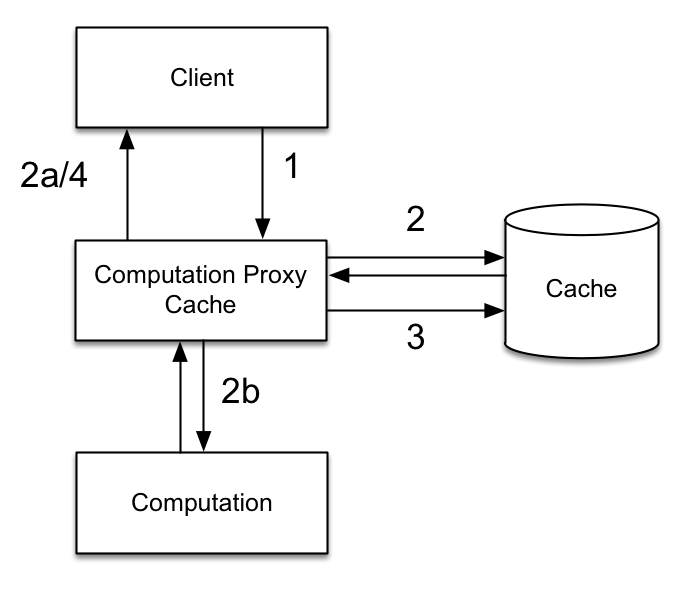
\includegraphics[width=0.6\linewidth]{figures/basic-caching-figure.pdf}
  \begin{enumerate}
    \item The result $v$ of a computation $f$ is requested.
    \item If $v$ is cached and is valid, we go to 5 with $v'=v$. Else we continue.
    \item We run the computation $f$
    \item The new result $v'$ of $f$ is stored in the cache.
    \item $v'$ is returned.
  \end{enumerate}
  \caption{The flow of basic caching}
  \label{fig:basic-caching}
\end{figure*}

In some cases, where the client is not allowed to wait for the computation to run, step 3-4 are replaced by a step that simply returns an empty value.

If we look at the cached value from an abstract point of view, we can see it as a \emph{result of a function} given certain \emph{inputs}. Sometimes the inputs are data from a storage system, sometimes it's the result of an API call to some external resource, sometimes it's global variables in the code. These \emph{inputs} we from now on be referred to as \emph{underlying data}.

In order for the algorithm to work, we need to be sure that when we store the cached value it has to be uniquely identified by some key such that when we lookup the value as in step 2 of the algorithm, we always locate $v$. This presents one of the challenges of cache management, which is in many cases closely related to cache invalidation (one of the two hard things in computer science\footnote{Not scientifically, but at least a favorite saying of Martin Fowler and quote by Phil Karlton}).

In the algorithm cache invalidation is simply described as a \emph{check}, but in reality this is the hard challenge of caching. The \emph{check} could be a precomputed indicator from earlier triggers, it could be based on a key derived from the underlying data or some timestamp. These cache invalidation approaches will be described more in section~\ref{sec:invalidation_techniques}.

\subsection{Architecture}
\label{subsec:architecture}

\begin{figure*}[ht!]
  \centering
  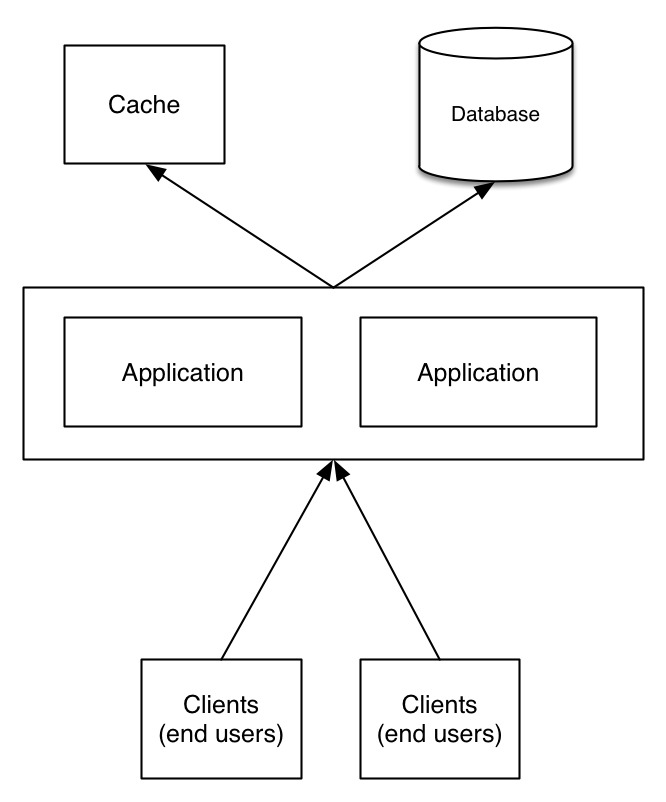
\includegraphics[width=0.5\linewidth]{figures/architecture.pdf}
  \caption{The assumed architecture of the system}
  \label{fig:caching-basics-architecture}
\end{figure*}

The architecture of the web application in which the cache is used is important to how the cache system. We assume that the architecture of the system is a common web application architecture as illustrated in figure~\ref{fig:caching-basics-architecture} consisting of a web application that serves HTTP-requests from the client (represented by the user) and interacts with a primary storage database to store and load data. To store and fetch the cached content we introduce a cache database. This could easily be the same unit as the primary storage database, but we separate them for better clarification.

Most modern web applications needs to serve multiple users at the same time, which means the web application must run on multiple processes\footnote{This is processes as an abstract term used in distributed systems. If we need to be implementation specific this could just as well be threads.} either on a single or multiple machines. We will therefore treat the web application as a distributed system.

A popular choice for cache databases are key-value stores such as Redis~\footnote{http://redis.io/} and Memcached~\footnote{https://memcached.org/} since they are simple distributed key-value stores that lives in memory and therefore allows for scalability and high-performance operations. In order to support most practical web applications, we will therefore make the assumption that the cache database has the same functionality: it should be possible to store arbitrary content for a given key. Furthermore the final solution of this thesis require the cache database to support atomic transactions for a given key, which are supported in Memcached using the CAS command~\cite{docs:memcached-protocol} and in Redis using the \verb$WATCH$-command~\cite{docs:redis-transactions}. The reasons behind this assumption will be explained more in chapter~\ref{chapter:update_propagation}.

% subsection architecture end

\subsection{Timeline Model}
\label{subsec:timeline_model}

As with the algorithm on figure~\ref{fig:basic-caching}, caching can be described by a series of events. The ordering of events decides whether the cached content or a fresh computation is presented to the client. To describe the different caching techniques, we will use a timeline model with a stream of events. One timeline describes the events occurring in a single process. We can therefore assume that there exists a total ordering of events for a single timeline. To be able to describe the caching techniques explained in this thesis, we will define the following events:

\begin{itemize}
  \item \textbf{Requested} is the event occurring when a client requests a given cached value
  \item \textbf{Computation Started} is when the computations is started
  \item \textbf{Computation Finished} is when the computation is finished and a result is returned
  \item \textbf{Stored} is happening when a given is stored in the cache database on a given key
  \item \textbf{UD Updated} is when the underlying data has been updated
  \item \textbf{Invalidated} is when the system has invalidated a cached value
\end{itemize}

To show how the timeline model works, we will give an example involving the different events:

\begin{example}
\label{example:timeline-model}
We will give an example using the basic caching algorithm described on figure~\ref{fig:basic-caching}. Consider the case illustrated on figure~\ref{fig:timeline-example}, where a client requests a value $v$ that at first isn't cached. This means the system will execute the function $f$, which returns the value instance $v_1$ and stores it in the caching database. After this some underlying data involving the computation of $v$ is updated and after the update, the client makes another request for $v$. At this point $v_1$ is not fresh since the execution of $f$ would result in another value. Therefore $v$ is invalidated by the system after which we recompute $f$ and stores the resulting value $v_2$ in the cache database.

\begin{figure*}[ht!]
  \centering
  % \includegraphics{width=1.0\linewidth]{figures/timeline-example.pdf}
  \caption{Example of the timeline model}
  \label{fig:timeline-example}
\end{figure*}

\end{example}

% Introduce the timeline and relevant events:
%   - Value registration
%   - Invalidation
%   - Cache update
%   - Value request
% Concurrent Timelines:
%   - Show that we when we have the given architecture, we have
%     multiple concurrent timelines running as in a distributed system
%     => We can assume that each timeline is a process

% TODO: Describe the model, when we know what to describe

% subsection timeline_model end

% section caching_basics end

\section{Evaluating Caching Techniques}
\label{sec:evaluating_caching_techniques}

% Goals of caching

To choose the correct caching technique for a given use case, we need to know the criteria for finally picking the best suited. The overall goal of caching in web development is to achieve a better user experience by getting a better performance and to save money by using less CPU power. If we assume that the cache system is able to retrieve cached values fast, the goals can be achieved by ``hitting the cache'' as often as possible. We can measure this using the metric \emph{cache hit rate}, which refers to the rate at which the cache is hit among the total number of requests for the cached value.

%% END CORRECTNESS

% Intro: from perspective of user

To evaluate the caching technique for a given use case, we will see the situation from the perspective of the client (i.e. a user). The client makes a request for some content that is served by the web server. This content contains of one or more computations that can be cached individually.

%%%% CONSISTENCY

We will not make any assumptions about the content send by the server, which means the content could be the result of multiple cached computations. Each of these computations are based on some underlying data e.g. served from the primary store. In the case where some computations are based on the same data we have to keep the different results consistent. Furthermore the response might be based on both cached content and content loaded directly from the primary store in which case we have to keep the data consistent across the cache database and the primary storage. This issue leads to the criteria of the level of consistency.

There exists multiple levels of consistency, but to keep it relevant and simple, we will evaluate the level of consistency using a binary value: either the caching technique ensures consistency with the data from the primary storage or else it doesn't.

%%%% FRESHNESS

Another parameter is the freshness of the content returned by the cache. It is most desirable to have content that is as fresh as possible as oppose to having stale data, but in the end the goal is to make the served content make sense for the user. Consider example~\ref{example:peergrade-split-interface} of the Peergrade.io platform, where there are two types of users. If the teacher changed the description of an assignment and a student requested and read the description 1 min after then it would not be unexpected behaviour to show the old description from the students point of view. On the other hand if the teacher requested the description 1 min after, it would be unexpected behaviour to show the teacher an old version, since the teacher would think the description hasn't been updated. We will represent freshness as a binary parameter that we call ``Strict Freshness'', which evaluates whether a given cached value that is fetched is guaranteed to be fresh.

\begin{example}
\label{example:peergrade-split-interface}
At Peergrade.io the web application has a teacher and a student interface. Teachers create assignments and sees statistics about the grades students have given to each other through their feedback. The students see the assignments created by their teachers, are able to hand in their assignments, and grade other students' hand in.
\end{example}


%%%% WAITING TIME AFTER INVALIDATION

While the freshness describes what is expected behaviour with relation to the content, there also exists time limits with relation to keeping the user focused on the task. Miller and Card et. al.~\cite{paper:miller-response-time-limit, paper:card-response-time-limit} describes these limits as:

\begin{itemize}
  \item When the response time is \textbf{0.1 second} the user feels that the system is \textbf{reacting instantaneously}.
  \item A response time above \textbf{1 second} will \textbf{interrupt the user's flow of thought}.
  \item \textbf{10 seconds} is limit related to \textbf{keeping the user's attention} on the given dialog.
\end{itemize}

In the basic caching algorithm described on figure~\ref{fig:basic-caching}, the computation has to run after it has been invalidated. If the caching technique runs this computation in the same process as the request from the client, the client has to wait for the computation to finish in order to show the content to the user. If the time taken to compute the value exceeds the accepted response time limits described above, it could become critical for the user experience. Based on this fact we will introduce the binary parameter of whether or not the client has to wait for the computation to finish after invalidation. The weight of this parameter is proportional to the cache miss rate since it's only requests, which results in a cache miss that are affected by the slow response time.

%%%% AUTOMATIC UPDATE/INVALIDATION

It is not possible to both serve the cached values immediately and have strict freshness. This can be proved using the example where a cached value is invalidated just before it is requested. We can only start computing the value at the moment it has been invalidated and given that the time between the invalidation and the request is smaller than the time taken to compute the value, it is not possible.

In cases where we choose immediate response time and we can tolerate serving cached values that are not strictly fresh, we might want to keep the cached values as up to date as possible. This means that we start computing the cached values as soon as they have been invalidated. In order to achieve this we need some mechanism that invalidates depending cached values when underlying data are updated. We will also represent ``Automatic Invalidation'' as a binary parameter.

%%%% CACHE MANAGEMENT

So far we've considered parameters from a user's perspective, but to evaluate the caching technique fully we also need to see it from the perspective of the developer since a big part of cache management is manually tracking dependencies between the cached content and the underlying data. We want the caching system to be transparent such that it is easy to add and remove caching from existing computations. Additionally we want the caching system to be robust such that when new code involving a cached computation is added, it should behave as expected without introducing errors. We cannot measure the level of robustness so we will therefore introduce the binary criteria: does the caching technique involve maintenance with relation to invalidation (shortened as invalidation maintenance)?

%%%% ADAPTABILITY

The last parameter we will introduce is also a requirement of the system: \emph{adaptability}. Since adaptability cannot be evaluated objectively we will introduce a scale of \emph{high}, \emph{medium} and \emph{low}, where high means that is adaptable to most systems and low means that it is adaptable to a few systems. We will define the scale as following:

\begin{itemize}
  \item \textbf{Low}: The technique has assumptions about the primary data store, cache database and/or application that means it cannot be applied to other common technologies.
  \item \textbf{Medium}: The technique is advanced and requires a lot of implementation effort or external libraries/processes to work.
  \item \textbf{Low}: The technique can easily be implemented and applied to existing applications.
\end{itemize}

The reason behind the \emph{Low} criteria is that when the technique has assumptions about the technology behind the application it means the system is tied to using specific technologies, which makes it difficult to change when the given technology is obsolete or the requirements of the system change. If this is not considered a problem \emph{Low} and \emph{Medium} can be considered the same level of adaptability.

From this discussion, we can sum up the evaluation parameters as follows:

\begin{itemize}
  \item \textbf{Consistency}: The cached value must be consistent with the other data
  \item \textbf{Strict Freshness}: The cached value must be as fresh as the state of the primary store when the value was requested
  \item \textbf{Automatic Update}: The cached value is automatically updated after it has been invalidated
  \item \textbf{Always Immediate Response}: The cached value must be served immediately after it has been requested
  \item \textbf{Invalidation Management}: Whether the developer has the responsibility of maintaining the invalidation of the cached values
  \item \textbf{Adaptability}: How adaptable the caching technique is to existing systems
\end{itemize}

% chapter caching_model end


\chapter{Caching Approaches}
\label{chapter:caching}

Many caching approaches for improving the throughput of web applications have been proposed. We discuss the approaches closest to the challenges of this thesis. The discussion will consider existing approaches with relation to the requirements for the system we design.

% TODO: Write some intro

\section{Invalidation Techniques}
\label{sec:invalidation_techniques}

One of the challenges of cache management is to maintain proper consistency between the underlying physical data and the cached data. If a cache system maintains strong consistency we know that when a cached value is read, it is a transformation of the most recent version of the underlying data it depends on. In the less strict model, weak consistency, it is only guaranteed that a cached value eventually becomes consistent with the most recent version of the underlying data.


% section invalidation_techniques end

\subsection{Expiration-based Invalidation}
\label{subsec:expiration_based_invalidation}

The requirement for strong consistency introduces complexity as seen with the trigger-based and key-based cache invalidation. Some objects can be cached with weak consistency, which allows much simpler caching techniques. One method is to assign a TTL (Time to Live) to the cached value. At some point when the TTL has expired, the cached object is invalidated. The invalidation can be enforced by the cache database (Redis and Memcached supports this - TODO: include references) or as part of the protocol between the client and server as with HTTP-caching explained in section~?~\cite{paper:web-caching-schemes}.

% subsection expiration_based_invalidation end

\subsection{Key-based invalidation}
\label{subsec:key_based_invalidation}

One method to achieve strong consistency is to use key-based invalidation when the cached value is requested. Key-based invalidation works by constructing the cache key from parts of the underlying data such that the when the cached object should change, then the key also changes.~\cite{blog:key-based-invalidation}. The cached content is considered immutable and only have to be written once. This simplifies version management from the perspective of cache storage since there is no chance you read stale values if the key is assumed to be derived from the most recent version of underlying data. The challenge of this method is to construct the key. In order for this caching method to work correctly, the developer must derive a cache key function f(x) such that the result of f(x) must be the same at any given time when given the same input x. In the web application framework, Ruby on Rails, the key construction is simplified by using a key that includes the timestamps of the last update on some underlying data. Although it simplifies the cache storage, the method also generates cache garbage, since old versions of a cached value are not removed. This means that the system relies on a cache database that is able to replace cache values using a proper policy such as replacing the Least Recently Used (LRU) or Least Frequently Used (LFU)~\cite{paper:web-caching-schemes}.


% subsection key_based_invalidation end

\subsection{Trigger-based Invalidation}
\label{subsec:trigger_based_invalidation}

Instead of invalidating the cached value when requested, the cached values can be invalidated based on certain triggers, which also guarantees strong consistency. This will make the code for requesting the cached value simpler, since the key used for storing the cached value does not have to update in lock-step with the underlying data.

The simplest triggers are write-through updates, which are manual triggers inserted by the developer at places where the cached values should be invalidated. This require all developers to keep track of all places where underlying data changes, and furthermore be sure that the manual triggers are inserted when new code is introduced.

In some architectures the changes to the system are based on triggers or events. One such architecture called Event Sourcing works by using Domain Events to describe the changes of the system instead of using database commands~\cite{blog:focusing-on-events}. Since these events are a natural part of the application, they can be used as invalidation triggers without further additions.

A lot of work has been put into using triggers from the database to invalidate cached data. \cite{paper:cache-genie} suggests a solution based on the Object Relational Mapper programming technique to capture relevant triggers. \cite{paper:deploy-time} also suggests using a database wrapper in the application-layer that captures and analyzes database commands and use them as triggers. TxCache suggested in~\cite{paper:liskov} uses daemon processes to monitor the database for relevant triggers. This method has the advantage that it allows multiple types of applications to manipulate the same database as opposed to~\cite{paper:cache-genie, paper:deploy-time}, where the triggers would not have been captured if the database command was made around the application. On the other hand it introduces complexity of running and monitoring the processes. With relation to database monitoring this introduces a trade-off between the complexity of the system and an assumption that multiple types of applications does not alter the same data.

% subsection trigger_based_invalidation end

\subsection{Automatic Invalidation}
\label{subsec:automatic_invalidation}

In~\cite{paper:liskov} Dan Ports et. al. uses database triggers to achieve transactional consistency for application-level caching, which ensures that any data seen within a transaction, shows a slightly stale but consistent snapshot across the storage and cache system. The database triggers are implemented using two database daemons that monitors a slightly modified version of PostgreSQL. The suggested solution, called TxCache, promises a very strong consistency guarantee, but it also comes with assumptions about the storage system and cache system used, and requires additional running daemons, which makes the full system more complex to run reliably. Furthermore these requirements contradicts flexibility and adaptability since the system assumes specific properties from the storage system and cache system, which makes it more difficult to change these components and adopt the caching system if an existing system does not use the given components.

Another solution proposed by Chris Wasik et. al.~\cite{paper:deploy-time} uses deploy-time analysis of the code to detect dependencies between the cached functions and the dependent relations. To invalidate the cached functions automatically, the system injects code that invokes relevant invalidation callbacks in places where the underlying data is updated. Where~\cite{paper:liskov} suggests a system that comes with requirements for the architecture and technologies used, the deploy-time model is a simple system that is able to use simple key-value stores for caching and any SQL storage system. But as oppose to~\cite{paper:liskov} it does not result in as strict consistency guarantees. But despite of being a simple method, the deploy-time model is based on a system where the source code changes for different environments, which could cause errors in one environment and not in others. As an example, the code in a development or test environment could work as expected but still result in errors when deployed to a production environment, where the code is injected. Even though the deploy-time solution avoids single points of failures as with a cache manager, it needs additional operations that have to be executed in the existing procedures. In a system with complex dependencies between the procedures and underlying data, the generated source code could decrease performance that cannot be optimized by the developer using the system.

CacheGenie is another cache system described by Priya Gupta et. al. that uses the Object Relational Mapping (ORM) library to detect changes made to the database. Some ORM libraries already implements these triggers, which makes this approach easier to integrate into web applications that uses ORM libraries, since the caching library does not rely on database monitors. CacheGenie tries to solve the problem of managing cache invalidation when caching database queries, by letting the developer predefine cached queries that are automatically updated in the application. CacheGenie is also based on a simple model, but each the cache definitions are based on assumptions about the specific queries and cannot be used to cache objects of a more coarse granularity.

On the other end of the granularity scale,~\cite{paper:db-driven-http} suggests a system that caches HTTP responses. It uses a sniffer process that monitors the lifetime of a HTTP request with the queries made to the storage system. Through the information captured by the sniffer, the system builds a table that maps a given HTTP resource to the queries made. The system then caches the HTTP resource that is invalidated when underlying data related to the given resource changes. This method is interesting since it allows to cache without changing the code of the web application, but it is only described at the granularity of HTTP responses since it uses the communication between the web application, storage system and cache to achieve automatic invalidation.

Jim Challenger et. al. has written multiple papers on the system used for the content management website in the Olympic Games in 1998 and 2000~\cite{paper:ibm, paper:ibm-extended}. The system is based on content that are all precomputed when served to the user, which resulted in a system that scaled for many users with content served fast since the web server only had to find the appropriate cached article when serving content. In order to allow editors to change articles and fragments, the system introduces the Data Update Propagation (DUP) algorithm. DUP uses an Object Dependence Graph (ODG) that describes the relationship between fragments using a Directed Acyclic Graph (DAG). The ODG describes both the relationships of how the fragments are embedded in each other and relationships describing the hypertext links between articles. To avoid race conditions and hypertext links to missing fragments, the fragments need to be updated in a specific order. More specific when a fragment f1 that embeds another fragment f2, the system need to update f2 before f1. Since the ODG is described DAG there is always a topological order of the nodes, which satisfies the described property for any node. The system runs using a CMS system, where the content is defined using a CMS system and not using functions from the source code. This simplifies the challenge of persisting the cached content since it does not change when a new version of the source code is deployed. It therefore leaves the challenge of updating cached content, when the definition of the computations changes.


% subsection automatic_invalidation end

\subsection{Hybrid Approaches}
\label{subsec:hybrid_approaches}

% TODO: Write something about combining different caching techniques to achieve satisfactory requirements

% subsection hybrid_approaches end

\section{Updating the Cache}
\label{sec:updating_the_cache}

% section updating_the_cache end

\section{Caching Approaches in Web Development}
\label{sec:caching_approaches_in_web_development}

% TODO: Rewrite this intro

One important aspect of caching is the granularity of the cached content. There is no doubt that it is most desirable to be able to cache any granularity, but since the cached content could be anything, the system cannot make any assumptions about cache management to e.g. allow for smarter invalidation. Therefore most existing work are based on a specific caching granularity from the data queried from the database to the HTTP response sent to the client.

\subsection{HTTP Caching}
\label{subsec:http_caching}

On the other end of the granularity scale, the developer could choose to cache the entire HTTP response send to the user. This could be the HTML documents served to the user as the website, but it could also be the JSON or XML response from an API. The HTTP protocol is the standard among web browsers to display web content and it’s widely used to communicate between web services. Since the HTTP protocol also include caching methods, which will be explained in the HTTP section, it is a very attractive caching technique among web applications.

The HTTP protocol includes multiple mechanisms for controlling cache consistency that allows the web server to implement both key-based and expiration-based cache invalidation. These mechanisms are controlled using HTTP headers. The expiration-based cache invalidation information about the cache date and age is specified using the Cache-Control header. The client is then able to derive if a given resource is valid at a given time or if the resource has to be refreshed. To use key-based invalidation, the web server can attach a tag that uniquely identifies a given version of a resources (e.g. using a hash of the content). When the client sends a new request, it attaches the ETag of the last version received, and the web server can now respond with a 304 Not Modified with no content. This tells the client it can safely use the last version.

Caching HTTP responses is a great technique when the same response are served to the multiple clients, but in situations where the content is updated often or personalized to each user, it becomes a less efficient technique since large documents are recomputed often. In the case where a small fragment of the content is personalized, it would be more desirable to only update that given fragment instead of recomputing the full document.

% subsection http_caching end

\subsection{Database Query Caching}

The database can be a bottleneck in the goal of achieving fast rendering of dynamic pages, because it’s often a requirement to have structured data at which you perform complex queries. In both cases the queries can become slow when the application need to scale with relation to data or users. Even though most storage systems allows indexing to optimize specific queries, it can still be difficult for the storage system to optimize in a space efficient way. One solution to this problem is to use query caches.

In~\cite{paper:transparent-caching, paper:cosar} this problem is solved using a proxy caching server between the web application and the database. This allows for transparent caching that require almost no changes to the system, but unfortunately it requires a lot of work to maintain the index used for cache validation and parse the queries received from the web application. Furthermore this solution are mostly made for relational databases with SQL language and require a new implementation for it to work on different storage technologies such as document-oriented databases.

\cite{paper:cache-genie} also describes a query caching solution, where the cache management is placed entirely in the application-layer. It is based on a common technology used in web application called Object Relational Mapper (ORM), where the data model is mapped to objects in the application and often the queries are made using methods on the object. Using the ORM in the Python framework Django, \cite{paper:cache-genie} implements an extension that allows common database queries to be cached and automatically updated. Compared to having a middleware caching layer, this solution has the advantage of being able to integrate with both different database technologies (within the capabilities of the ORM) and caching systems. On the other hand, it does not capture database updates made without using the ORM. This means if updates are made manually or another application uses the same database, the cached queries are not updated.

\subsection{Materialized Views}

Where the query caches described so far are either middle-tier or on the application-layer, caching using materialized views occurs on the database layer. Materialized views are “virtual tables” generated from other data in the database. It works by storing queries explicitly declared by the developer. The virtual tables can be explicitly refreshed or update when the dependent data changes. Materialized views is a good solution for optimizing database queries, but since the computation occurs on the database level, the computation capabilities are limited by the database technology.

Caching database queries and materialized views allows for easy and transparent caching, but it does not allow computations on the web application, which limits the applicability.

% section caching_approaches_in_web_development end


\subsection{Function Caching}

% TODO: Find another place for this text, please.

A more flexible technique is to cache functions. \cite{paper:liskov} describes a programming model for cacheable functions that essentially is functions annotated as cacheable. Although this seems attractive, it has limitations with respect to the procedures executed in the function. \cite{paper:liskov} describes the requirement of cachable functions of their programming model: “To be suitable for caching, functions must be pure, i.e. they must be deterministic, not have side effects, and depend only on their arguments and the storage layer state.” By this definition they explain that the storage layer state are treated as implicit arguments and thereby reach the classical definition of a pure function that is a transformation that always gives the same output from the same input.

\cite{paper:deploy-time} suggests a similar programming model, where the relationships of the underlying data has to be explicitly annotated, but where the rest of the caching system is much simpler than the one described in~\cite{paper:liskov}.

The requirement for strong consistency introduces complexity as seen with the trigger-based and key-based cache invalidation. Some objects can be cached with weak consistency, which allows much simpler caching techniques. One method is to assign a TTL (Time to Live) to the cached value. At some point when the TTL has expired, the cached object is invalidated. The invalidation can be enforced by the cache database (Redis and Memcached supports this - TODO: include references) or as part of the protocol between the client and server as with HTTP-caching explained in section~\cite{paper:web-caching-schemes}.

% subsection function_caching end

\section{The Problem of Incorrect Write-Through}
\label{sec:the_problem_of_incorrect_write_through}

% TODO: Write this as a problem that is ignored in many existing caching solutions or maybe just traded off for simplicity. Describe how key-based invalidation ensures this and how all other could have this problem solved.

At first we would like the caching to be correct. In the case of caching, we will define correctness in terms of liveness and safety: the caching system will update the cache when necessary and it will eventually return the most fresh value computed. That is if we have a computation $f$ that computes the value $v_1$ at time $t_1$ and $v_2$ at time $t_2$ then the cache store will eventually contain $v_2$ given that $t_2 > t_1$. Although this could be seen as a prerequisite for the caching system, most implementations ignore this fact to achieve a simpler cache system. Because when we want to keep the integrity between updates we need some kind of ordering for the updates that adds complexity to the system. The problem is also illustrated on figure~\ref{fig:incorrect-updates-analysis}.

\begin{figure*}[ht!]
  \centering
  \includegraphics[width=1.0\linewidth]{figures/incorrect-update-analysis.pdf}
  \caption{Showing how two concurrent caching updates from two different application servers results in an inconsistent state. We see that even though the request from \emph{Web 2} are based on data older than \emph{Web 1} it gets to write }
  \label{fig:incorrect-updates-analysis}
\end{figure*}

% TODO: Analysis and argue why some of the solutions leads to inconsistent cached values and breaks the safety requirement.

% section the_problem_of_incorrect_write_through end

\section{The Trade-Off between Consistency, Freshness and Immediate Response}
\label{sec:the_trade_off_between_consistency_freshness_and_immediate_response}

% TODO: Write that you cannot have all three at the same time

% Choosing: Consistency and Freshness:
%   - Consider the following case:
%     - A client makes a request that invalidates $v$ at time $t1$
%     - Another client makes a request for getting value $v$ at time $t2$

% section the_trade_off_between_consistency_freshness_and_immediate_response end



\section{Choosing the right Caching Technique}
\label{sec:choosing_the_right_caching_technique}

% Write a lot about the trade-offs:

The system need to cache the result of computations, which means it has to cache objects with a granularity more coarse than database queries. The HTTP protocol includes multiple features for cache management between the client and server, but it also makes the caching inflexible with relation to efficiency. In some situations HTTP responses includes shared fragments that need to be computed for each HTTP endpoint. Since the system expects long running computations, it would be more efficient to cache the result of those computations, meaning the system need to work on a granularity of fragments or functions. Since functions returns an output that could be considered a fragment, we will consider them as the same granularity.

In order to keep the cached values up to date we need automatic cache invalidation. In order to achieve automatic cache invalidation with transactional consistency,~\cite{paper:liskov} describes a solution a solution that need assumptions about the storage and cache system. The system designed in this thesis does not need such strict consistency guarantees, and some of the components in the solution is therefore not necessary.

The solution suggested by Jim Challenger et. al. is highly relevant to the problem of this thesis, but since the system is designed for a publishing system, it leaves some challenges that have to be solved to satisfy the requirements of this thesis.

Also relevant is the paper by~\cite{paper:deploy-time} that suggests a solution that identifies dependencies and injects invalidation callbacks into the source code on deployment. This method makes the caching transparent, but it also comes with the cost that the code will be different in development and production. Furthermore the solution described does not perform write-through updates, which would also be inefficient since it would slow down existing operations that involved cache invalidations.

Conclusion from this chapter: solutions exists for a lot of the sub-problems this thesis is facing, but there exists no complete solution to satisfy the requirements.

% section choosing_the_right_caching_technique end

\chapter{Smache: Cachable Functions}
\label{chapter:smache-cachable-functions}

The goal of this thesis is to present a caching solution that is able to handle long running computations by presenting content to the user fast while addressing the challenges of cache management and efficient update propagation. This chapter will present the overall solution suggested by the thesis.

In this chapter we will start by arguing why the existing caching approaches are not sufficient (section~\ref{sec:existing-approaches-are-not-sufficient}). Followed by these arguments, we present the programming model that is the basis of the solution (section~\ref{sec:the_cachable_function_model}), how we implemented this model in Python (section~\ref{sec:implementing_cachable_functions_in_python}), and a final discussion on the limitations of the design and implementation of the model (section~\ref{sec:cachable-function-discussion}).

\section{Why Existing Approaches are Not Sufficient}
\label{sec:existing-approaches-are-not-sufficient}

In the primary use case of the context in this thesis (described in section~\ref{sec:context}), the platform presents statistical information based on some advanced computation that takes a long time to compute ($>\text{ 10 sec.}$). If we want to keep the teacher's attention to the platform, we need to find a caching technique, where the response time does not depend on the computation time. Furthermore we want to keep the information as fresh as possible.

If we consider the overview on figure~\ref{fig:existing-solutions-comparison}, we can already leave out caches that optimize DB-queries and declared content since they do not solve the problem of caching advanced statistical computations. The solution proposed by IBM is made for declared HTML-content and not on computations based on data from a storage system. This leaves the set of approaches that are able to cache arbitrary content and HTTP-responses, but given caching arbitrary content has less assumptions, they are more attractive.

From the approaches caching arbitrary content it is desirable to have an approach with high adaptability, which is one of the requirements of the system. From the approaches with high adaptability, which has a response time that does not depend on the time of computation, are \emph{expiration-based} and \emph{manual trigger-based invalidation with asynchronous updates}.

From these approaches the expiration-based invalidation technique has the advantage that it doesn't require much invalidation management, but it has the limitation that all cached values of the same kind are invalidated and updated at the same frequency.

If we consider use case example~\ref{example:assignment-computations}, the statistical information of current assignments would be updated at the same frequency as the closed assignments, and if we want to keep the cached values for the current information up to date, we also need to update all non current information. This is not desirable with relation to efficiency since the CPU will be busy in time proportional to the taken to compute the statistical information for the assignment and the total number of assignments on the platform. In other words the number of CPU's we need to occupy for this job can be calculated by $\frac{\Delta t_c \cdot n_c \cdot u_c}{t_d}$, where $\Delta t_c$ is the time taken to compute a single assignment, $n_c$ is the number of assignments, $u_c$ is the number of updates per 24 hours, and $t_d$ is the number of seconds per 24 hours. Considering the example - if we have 500 assignments on the platform and we want to update the information every 10 minutes with a computation time of 30 seconds each, then we get $\frac{30 \cdot 500 \cdot \frac{60}{10} \cdot 24}{60 \cdot 60 \cdot 24}\text{ occupied CPU's} = 25\text{ occupied CPU's}$. If the amount of computational power isn't a problem, the expiration-based approach would be the best solution, but that is not the case of this thesis, where efficiency is a requirement.
$\frac{30 \cdot 500 \cdot \frac{60}{10} \cdot 24}{60 \cdot 60 \cdot 24}\text{ occupied CPU's} = 25\text{ occupied CPU's}$. If the amount of computational power isn't a problem, the expiration-based approach would be the best solution, but that is not the case of this thesis, where efficiency is a requirement.

The last alternative with high adaptability is to use manual trigger-based invalidation with asynchronous updates after request as described in section~\ref{subsec:trigger-based-invalidation-with-asynchronous-update}. This approach has the advantage that the values are only invalidated (and thereby recomputed) when a trigger is invoked, which means the programmer has the opportunity to optimize the approach to only invalidate when it is relevant to the user e.g. when the cached value are supposed to change. Although this can be seen as an opportunity it can also be seen as a burden for the programmer to maintain these manual triggers. Furthermore by having asynchronous invalidations, the user is always presented with a stale value on the first request after invalidation. If we consider example~\ref{example:assignment-computations} it is not unlikely that the teacher looks at an old assignment some time after it has been closed, which might just be a single request. In this case, the cache system would serve a stale value and update the value without purpose.
\begin{example}
\label{example:assignment-computations}
On the Peergrade.io platform the teacher is presented with statistical information about the grades given by the students for a given assignment. These assignments are often current at specific time interval after which the assignment becomes ``closed'' and the statistical information are not updated.
\end{example}
The approaches suggested by Chris Wasik and Dan Ports focus on automatic invalidation and could probably be extended to do asynchronous updates on request to allow immediate responses by giving up the option of freshness, which would give the same guarantees as the trigger-based invalidation with asynchronous updates, but it would also have the same challenges.

The deploy-time model~\cite{paper:deploy-time} and TxCache~\cite{paper:liskov} chooses consistency over ensuring immediate response times and are therefore not suitable for long running computations. TxCache shows how it achieves a higher cache hit rate by limiting the number of recomputations in each request, but it does not reach 100\% hit rate. The deploy-time model could be extended to have immediate response time by using write-through invalidation, but it uses static invalidation, which is highly coupled to the specific technology, and makes it difficult to change technologies.

The approach best fit for the context of this thesis is to use write-through invalidation that guarantees immediate response time as well as updating the content in-place such that the content cannot become older than the time taken to compute the value. Although this is the best fit, it still leaves a burden for the programmer to declare the triggers that invokes the write through updates as well as naming the cached objects. Furthermore it leaves the challenge of ensuring the integrity of the cached values and invalidation marks in concurrent environments as described on figure~\ref{fig:trigger-based-concurrency-problem}.

The goal of the thesis is to design a solution that is easy for existing applications to adapt and support caching long running computations. To support long running computations the cache must be able to serve slightly stale values to serve the result immediately, while keeping the result up to date in an efficient way. As we can see on figure~\ref{fig:existing-solutions-comparison}, there exists no solutions fulfilling those criteria, and we will therefore suggest a new solution, which we call ``Smache''.

In the rest of this thesis we will describe the design and implementation of ``Smache''.

% section existing-approaches-are-not-sufficient end

\section{The Cachable Function Model}
\label{sec:the_cachable_function_model}

Smache uses an extended version of the programming model described by Dan Ports~\cite{paper:liskov}. The model is organized around \emph{cachable functions}, which essentially are normal functions, where the result are \emph{memoized}\footnote{In our case: storing the result of the function and return the cached value when the function is called again with the same input}. The cachable functions are allowed to make request to the primary storage to fetch the underlying data as well as calling other cached functions. This allows caching at different granularities that gives the benefit of optimizing the invalidation for different types of content.

% - Definition of cachable function (taken from Dan Ports)

\subsection{Restricted to Pure Functions}
\label{subsec:restricted_to_pure_functions}

As mentioned by Dan Ports~\cite{paper:liskov} not all functions are cachable. To be able to cache the functions they need to be \emph{pure}, which Dan Ports defines as: \myquote{[...] they [functions] must be deterministic, not have side effects, and depend only on their arguments and the storage layer state.}. Smache does not detect these properties in a function and therefore relies on the programmer to ensure only pure functions are cached.

% subsection restricted_to_pure_functions end

\subsection{Making Functions Cachable}
\label{subsec:making-functions-cachable}

Smache has automatic invalidation, but it is only semi-transparent, since that relies on the programmer declaring dependencies to underlying data. The API for making functions cached is defined as following:

\verb$MAKE-CACHABLE(fn, input-types, relation-deps)$ $\rightarrow$ \emph{cached-fn}: Makes a function cacheable. \emph{cached-fn} is a new function that first checks the cache for the result of another call with the same arguments. If not found, it executes \emph{fn} and stores its result in the cache.

The added arguments for the procedure does not alter the behaviour of the \emph{cached-fn}, but it requires additional arguments used by the application for naming and invalidation. The \emph{input-types} are the types of the arguments (e.g. the type of entity or type of raw content) given to the original \emph{fn} and the \emph{relation-deps} are declared dependencies to data sources, which cannot be derived from the input of \emph{fn}. The \emph{input-types} are used to indicate how the arguments should be interpreted with relation to naming (described in section~\ref{subsec:cache-object-localization}) and used together with the \emph{relation-deps} to achieve automatic invalidation (described in chapter~\ref{chapter:invalidation}).

% subsection making_functions_cachable end

\subsection{Cache Object Localization}
\label{subsec:cache-object-localization}

When the application fetches and stores cached objects, the developer must derive a name that is used as the key in the cache store and for identifying the cached object. To localize a cached object correctly the name \emph{must be unique} such that no other cached function is able to have the same name. To make it easier for the programmer to cache functions, Smache automatically generates the name based on the input given to \verb$MAKE-CACHABLE$. The localization uses the \verb$SERIALIZABLE-FUN-NAME$ procedure that is defined as following:

\verb$SERIALIZABLE-FUN-NAME(fn, input)$ $\rightarrow$ \emph{fun-name}: Returns the name that uniquely identifies the cached object instance representing the call to the function \emph{fn} with \emph{input}. The name is constructed by concatenating a unique serialized version of \emph{fn} and a serialization of the \emph{input}. The serialization of \emph{input} is done by concatenating a serialized version of each argument.

This procedure makes it possible to represent the cached object in the cache to locate and store the result of a given cached function in the cache database.

To support asynchronous write-through updates that allows the cache system to automatically update the cached objects as they are invalidated,
\verb$SERIALIZABLE-FUN-NAME$ must also comply with the following requirement:

\begin{itemize}
  \item The serializations of \emph{fn} and \emph{input} must be done in such a way that there exists another procedure \verb$DESERIALIZE-FUN$ that deserializes \emph{fun-name} such that it is possible to locate and call \emph{fn} with \emph{input} in another process.
\end{itemize}

The \verb$DESERIALIZED-FUN$ is defined as following:

\verb$DESERIALIZED-FUN(fun-name)$ $\rightarrow$ \emph{fun}, \emph{input}: Returns a pointer to \emph{fun} as well as the original \emph{input}. It must be possible to call \emph{fun} with \emph{input} as arguments such that the result is the same as before \verb$SERIALIZABLE-FUN-NAME$ was applied.

% subsection cache-object-localization end

\subsection{Automatic Cache Invalidation}
\label{subsec:automatic_cache_invalidation}

Dan Ports' TxCache~\cite{paper:liskov} handles all parts of cache management transparently such that the programmer only have to define which functions needs to be cached and not define how it should be invalidated. This is a great advantage since it avoids potential bugs related to cache invalidation, but it is a trade-off for flexibility as well as adaptability since this approach moves the complexity to the database in the form of assumptions about the primary storage, cache database, and requires an external daemon process for managing snapshots~\cite{paper:liskov}.

Smache does not remove the burden of cache management, but it will handle naming (or localization) and invalidation by only relying on the programmer declaring dependencies to underlying data. This will improve the usability of cache management since the cache invalidation only changes when there are changes to the underlying data as described more in chapter~\ref{chapter:invalidation}.

% subsection automatic_cache_invalidation end

\subsection{Write-Through Invalidation}
\label{subsec:write-through-updates}

Smache also offers the possibility to perform write-through invalidation using a data update propagation system inspired by the solution IBM used to achieve a 100\% cache hit rate on the content management system for the Olympic Games in 2000~\cite{paper:ibm, paper:ibm-extended}.

Having write-through invalidation allows the programmer to achieve immediate response times while ensuring that the values returned are updated as soon as they are invalidated, such that the value is not more stale than the time taken to compute it. This will be explained more in chapter~\ref{chapter:data-update-propagation}.

% subsection write-through-updates end

\section{Implementing Cachable Functions in Python}
\label{sec:implementing_cachable_functions_in_python}

% How the cachable function works
Smache implements the cachable function by exposing an implementation of the \verb$MAKE-CACHABLE$ to the programmer. To apply the procedure the Smache library must be loaded in the application and applied. The \verb$MAKE-CACHABLE$ converts the original function to a cached function that intercepts the method invocation and directs it to a wrapper function in the Smache library. When a client makes a request involving a cached function, the application will call the function wrapper that tries to find the value in the cache first and if it is not present in the cache, the original function will be called after which the result is cached and returned to the caller. This control flow of a cached function is illustrated on figure~\ref{fig:cachable-function-control-flow}.

\begin{figure*}[ht!]
  \begin{center}
    \includegraphics[width=1.0\linewidth]{figures/cachable-function-control-flow.png}
  \end{center}
  \begin{enumerate}
    \item The caller invokes the cached function through the cached wrapper in Smache
    \item Smache sends a \verb$Lookup$ request to the Cache Database
    \item The cache database returns a cached object instance
    \item[(4)] Smache calls the original function through the application
    \item[(5)] The application executes the original function, makes the necessary calls to the primary storage and returns the result
    \item[(6)] Smache sends a \verb$Store$ request to the Cache Database with the result from the application
    \item[7] Smache returns the value to the caller from the application
  \end{enumerate}
  \footnotesize{Steps annotated with \emph{parenthesis and dashed lines} are only executed in case of cache miss or cache failure}
  \caption{The control flow during a call to a function cached through Smache}
  \label{fig:cachable-function-control-flow}
\end{figure*}

The procedure for making a function cached is implemented using Python-decorators~\footnote{https://www.python.org/dev/peps/pep-0318/}, which is an annotation used to modify the behaviour of existing functions while being able to keep a reference to the original function.

Code snippet~\ref{code:basic-caching-running-example} shows how the decorators are applied to the running example. The only addition we have made is a call to a function called \verb$computed$ on a module \verb$smache$ with a single argument and a \verb$@$ as prefix that indicate it is a decorator. Additionally there is a decorator called \verb$relation$ in which we indicate the entity type as well as a function that describes how the given relation entity relates to an entity indicated through the input. This call corresponds to the implementation of \verb$MAKE-CACHABLE$, where the arguments given to \verb$computed$ are the \verb$input-types$ and the arguments given to \verb$relation$ are the \verb$relation-deps$.

\begin{code}{How to cache the functions from the running example using Smache.}
  \input{code/basic_implementation.py}
  \label{code:basic-caching-running-example}
\end{code}

% Declaration
Smache require the programmer to annotate the types of ``underlying data'', which are passed into the original function. In this case we have annotated using the \verb$Course$-class that corresponds to an object for an Object-Relational Mapper (ORM) that represents the collection \emph{course}. The ``underlying data types'' supported are ORM-objects as well as the ``Raw''-type that represents primitive values (such as strings, numbers etc.). The number of type annotations has to be the same number of arguments given to the original function. The type annotations are used to derive direct dependencies as explained more in section~\ref{chapter:invalidation} and to implement automatic naming.

% Naming
The Smache library implements both the \verb$SERIALIZED-FUN-NAME$ and \verb$DESERIALIZED-FUN$ to support automatic write-through invalidation. The implementation works by having a \emph{seperator-token} that is used in between the concatenations. The input is deserialized and serialized using the \emph{JavaScript Object Notation}-protocol (JSON)~\cite{docs:json}. Using the python implementation~\cite{docs:python-json} Smache encodes primitive Python values into JSON and decodes them back from JSON to Python values. The implementation of the encoding and decoding can be seen in appendix~\ref{appendix:implementation-of-function-serialization-and-deserialization}. Besides decoding and encoding the cached object instances, the full implementation also involves storing and loading references from/to the computed functions.
To give an example, we will demonstrate the usage of the localization procedures with the default seperator token \verb$~~~$. We can serialize the function \verb$course_score$ from the running example in code~\ref{code:running-example}. When the running example has been made cachable as in code~\ref{code:basic-caching-running-example} and we use a \verb$Course$-instance from the \verb$ORM$ we can serialize and deserialize as seen in code~\ref{code:function-serialization}.

\begin{code}{Example of how function serialization and deserialization can be done in Smache}
  \input{code/function_serialization.py}
  \label{code:function-serialization}
\end{code}

% section implementing_cachable_functions_in_python end

% section the_cachable_function_model end

\section{Limitations of Cachable Functions}
\label{sec:cachable-function-discussion}

The design of the cachable functions require the programming language to support serialization and deserialization as described. In Python it is possible to localize modules and functions dynamically based on a string representation, but in other languages this could be a challenge or might even require a different solution, which could be a limitation of both the design and implementation. For example statically typed languages that does not allow dynamic notations, might need a different solution, where the representations are mapped to a data structured holding references to the given functions. Furthermore the solution does not consider caching methods for objects in object oriented languages. To cache methods of objects, the solution would have to be extended to consider the state of the object as ``input'' for the cached function.

Another limitation of the interface of cachable functions described so far is that it is only possible to use it for trigger-based invalidation and the only control for the programmer is to define the dependencies such that the cached object is invalidated appropriately. There could be cases, where the cached object were to be invalidated based on some data sources, but also be updated once every day using expiration-based invalidation. Fortunately, the interface can easily be extended using decorators to include optional parameters that would allow hybrid approaches such as these.

% section discussion end

\section{Summary}
\label{sec:cachable-functions-summary}

In this chapter we argued why existing approaches does not solve the problem addressed in this thesis and presented the programming model for the suggested solution. We introduces the interface for \emph{cachable functions} that allows a programmer to declare a function to be cached. When a cached function is called the second time with the same input, the result will be served from the cache. The naming and identification of the related cached object instance is handled transparently by the caching system. The interface also includes declaration that allows cachable functions to be extended with automatic invalidation as described in the next chapter (chapter~\ref{chapter:invalidation}) and write-through invalidation (chapter~\ref{chapter:data-update-propagation}).
The programming model has been implemented in Python, where the declaration for caching a function is implemented using decorators. The serialization and deserialization is implemented by encoding the function and input into JSON and decoded back into a pointer to the function and Python values. This procedure might be a limitation for dynamic languages such as Python.

% section summary end

% chapter smache-cachable-functions end

\chapter{Automatic Cache Invalidation}
\label{chapter:invalidation}

In the model for cachable functions described in the previous chapter~\ref{chapter:smache-cachable-functions} we've only described how the system can make a function cachable such that Smache automatically stores and locates the cached object returned by the function. While this removes the burden of naming and localizing cached objects, it does not solve the hard problem of invalidation.

To make cache invalidation easier with Smache, we will extend this solution with an invalidation mechanism that automatically invalidates the cached objects based on dependencies declared by the programmer.

This chapter describes how the suggested system uses the declared dependencies to track updates to underlying data and invalidate cached objects correctly. The solution for automatic invalidation is described in three parts. First we introduce the data structures used to achieve fast and efficient invalidation (section~\ref{sec:simple-object-dependence-graph}). Second, the \emph{dependency registration} describes how the cached objects are registered into the ODG. Finally, the \emph{invalidation propagation algorithm} (section~\ref{sec:invalidation-propagation} describes how Smache invalidates affected cached objects when changes are made to the underlying data. The chapter ends with a discussion on how the suggested solution meets the criteria and requirements of the thesis.

% section dependency-registration end

\section{Simple Object Dependence Graph}
\label{sec:simple-object-dependence-graph}

The Object Dependence Graph (ODG) was first described in a series of papers by IBM~\cite{paper:ibm, paper:ibm-extended} and was build to support the content management system build for the Olympic Games in 2000. The final content served to the user is build from HTML-fragments and HTML-pages editable by the users as well as underlying data periodically changing. To be able to serve the final documents fast, the system pre-generates the HTML pages such that the system doesn't have to generate the pages on each request. To do this efficiently, the system maintains dependencies between the different kinds of objects and updates depending objects when underlying data changes. The cache object pre-generation can also be described in terms of caching, where the system uses an in-place caching approach.

Jim Challenger et.al.~\cite{paper:ibm-extended} presents a simple and a generalized version of the ODG. The generalized version is described for a content management system and includes a number of enhancements compared to the simple model that is unnecessary for the purpose of this thesis. We will therefore use the simple ODG that is described as following:

ODG can be represented using a directed graph, where a vertex either represents underlying data or an object that is a pure transformation of underlying data. An edge from a vertex representing underlying data $u$ to a vertex representing an object $o$ denoted ($u$, $o$) indicates that a change to $u$ also affects $o$.~\cite{paper:ibm-extended} gives the following constraints for the simple ODG:

\begin{itemize}
  \item Each vertex representing underlying data does not have an incoming edge
  \item Each vertex representing an object does not have an outgoing edge
  \item All Vertices in the graph correspond to underlying data (nodes with incoming edges) or objects (nodes with an outgoing edge)
  \item None of the edges have weights associated with them
\end{itemize}

Figure~\ref{fig:simple-odg} illustrates an instance of a simple ODG with four vertices of underlying data ($u_1$, $u_2$, $u_3$ and $u_4$), two vertices representing objects ($o_1$ and $o_2$), and the dependencies between them. Where we can see that when underlying data $u_2$ changes, the system must update both the cached object of $o_1$ and $o_2$ and when $u_4$ changes, it only needs to update $o_2$.

\begin{figure*}[ht!]
  \centering
  \includegraphics[width=0.6\linewidth]{figures/simple-odg.pdf}
  \caption{An example instance of a simple ODG}
  \label{fig:simple-odg}
\end{figure*}

% section simple-object-dependence-graph end

\section{Dependency Data Structure for Cachable Functions}
\label{sec:dependency-data-structure-for-cachable-functions}

There exists two representations of dependencies for cachable functions. The first one is the static representation, which can be derived directly from the declarations in the source code. This representation only describes dependencies between the declarations and not cached object instances. We will define this representation as the \emph{Declaration Dependence Graph (DDG)}. The other representation is dynamic and describes the dependencies between the entities of the underlying data and the cached object instances. We define this as the \emph{Instance Dependence Graph (IDG)}.

\subsection{Declaration Dependence Graph}
\label{subsec:declaration-dependence-graph}

When the cachable functions are defined as in section~\ref{subsec:making-functions-cachable}, the dependencies are declared using the entity types. The DDG is an extension of the Simple Object Dependence Graph, where the cached functions corresponds to the object vertices and the entity types corresponds to the underlying data. Where the simple ODG only includes direct dependencies, the DDG has two kind of dependencies. An edge from $u$ to $o$ denoted $(u, o)_d$ represents a direct dependency, which means that the dependency defines the given $o$. That is if a given cached object instance has a dependency to an instance of an entity then it cannot change. The direct dependencies includes an index indicating a position such that there is an order of direct dependencies for a given cached object. An edge from $u$ to $o$ denoted $(u, o)_l$ represents a lazy dependency, which means that the dependency can change throughout the lifetime of the cached object instance and has to be evaluated before invalidation to derive the dependency for the instance. This could just as well be two graphs, but we model it as one for illustrative purposes.

Figure~\ref{fig:declaration-dependence-graph} shows the DDG for the running example from code snippet~\ref{code:running-example}. For example we see that the cached object for the \verb$participant_score$-function depends directly on the participant and it depends lazily on the grade. This is because there exists a participant for each score, but the dependencies from a cached object instance to any grade entity can change throughout the lifetime.

\begin{figure*}[ht!]
  \centering
  \includegraphics[width=0.6\linewidth]{figures/declaration-dependence-graph.pdf}
  \caption{The Declaration Dependence Graph of the running example}
  \label{fig:declaration-dependence-graph}
\end{figure*}

The DDG graph is represented using two data structures. The lazy dependencies are represented using an outgoing adjacency list from the underlying data nodes. The direct dependencies are represented using an incoming adjacency list from the object nodes ordered by the position index of the dependency. To access a given adjacency list fast we use hash tables index by entity type for the outgoing adjacency list and by the object ID for the incoming adjacency lists as depicted on figure~\ref{fig:ddg-data-structure}.

\begin{figure*}[ht!]
  \centering
  \includegraphics[width=0.6\linewidth]{figures/ddg-data-structure.pdf}
  \caption{An illustration of the data structure representing the DDG on figure~\ref{fig:declaration-dependence-graph}}
  \label{fig:ddg-data-structure}
\end{figure*}

New dependencies can be added to the DDG using

\begin{itemize}
  \item \verb$add_dependency(s_id, t_id)$: Adds a dependency between the source id \verb$s_id$ used as index for the hash table and the target id \verb$t_id$ used as element in the adjacency list.
\end{itemize}

When \verb$add_dependency$ is used we check if there already exists an adjacency list in the hash table using \verb$s_id$. If there exists one, we add \verb$t_id$ to the given adjacency list, or else we add a new adjacency list only including \verb$t_id$ and indexed by \verb$s_id$.

The DDG is build by iterating through all the cached functions with their respective dependencies and add the dependencies to the data structure as described above. The lazy dependencies are added with the entity type as \verb$s_id$ and the cached function as \verb$t_id$. The direct dependencies are added using the cached function as \verb$s_id$ and the entity type as \verb$s_id$.  The advantage of the DDG is that it does not change in the lifetime of the application, which means it can be preprocessed when the application starts.

The queries needed for automatic cache invalidation are the following:

\begin{itemize}
  \item \verb$lookup_lazy_dependency(entity_type)$: Finds all lazy dependencies from a given entity type
  \item \verb$lookup_direct_dependency(fun_id)$: Finds all direct dependencies from a given function id
\end{itemize}

Using these data structures we can access a pointer with access to all lazy or direct dependencies using $O(1)$ expected time if we use a hash table using perfect hashing.~\cite{paper:perfect-hashing}. In worst case the space used is the maximum number of edges $O(|u| \cdot |o|)$, where $|u|$ denotes the number of notes representing underlying data and $|o|$ represents the number of nodes representing objects.

% subsection declaration-dependence-graph end

\subsection{Instance Dependence Graph}
\label{subsec:instance-dependence-graph}

The Instance Dependence Graph (IDG) is also an extension of the simple Object Dependence Graph (ODG), where the data entities corresponds to underlying data and the cached object instance generated from the cachable functions corresponds to the objects. An edge from underlying data $u$ to an object $o$ denoted ($u$, $o$) indicates that if $u$ is changed then $o$ must be updated.

The instance dependence graph for the running example is illustrated on figure~\ref{fig:instance-dependence-graph}. In the given example, this graph is quite primitive. It's worth noting that the edges in the IDG are instance specific representations of the direct dependencies of the DDG seen on figure~\ref{fig:declaration-dependence-graph}.

\begin{figure*}[ht!]
  \centering
  \includegraphics[width=0.3\linewidth]{figures/instance-dependence-graph.pdf}
  \caption{An example of an Instance Dependence Graph based on the running example}
  \label{fig:instance-dependence-graph}
\end{figure*}

The representation of the IDG is similar to the representation of lazy dependencies for the DDG, where the dependencies are represented using an outgoing adjacency list indexed by a hash table as illustrated on figure~\ref{fig:idg-data-structure}.

\begin{figure*}[ht!]
  \centering
  \includegraphics[width=0.6\linewidth]{figures/idg-data-structure.pdf}
  \caption{An illustration of the data structure representing the IDG on figure~\ref{fig:instance-dependence-graph}}
  \label{fig:idg-data-structure}
\end{figure*}

New dependencies are added using \verb$add_dependency$ described for the DDG in section~\ref{subsec:declaration-dependence-graph}, where the entity id is the source and the cached object is the target.

The queries needed for automatic invalidation are:

\begin{itemize}
  \item \verb$lookup_cached_object(entity_id)$: Finds all cached objects depending on the \verb$entity_id$.
\end{itemize}

% subsection instance-dependence-graph end

% section dependency-management-for-cachable-functions end

\section{Dependency Registration}
\label{sec:dependency-registration}

For the application to know what and when to invalidate, the application must register the dependency declarations and name of cached functions instances. The dependency declarations that defines the lazy and direct dependencies are part of the source code and therefore available when the application is started as illustrated on figure~\ref{fig:declaration-dependency-registration}. This registration flow simply collects all the cached functions registered through the cachable function procedure and adds them as dependencies in the DDG.

\begin{figure*}[ht!]
  \centering
  \includegraphics[width=1.0\linewidth]{figures/declaration-dependency-registration.pdf}
  \caption{The flow in which lazy and direct dependencies are registered from the declarations}
  \label{fig:declaration-dependency-registration}
\end{figure*}

The registration of cached object instances happens when the cached object is accessed for the first time as illustrated on figure~\ref{fig:instance-dependency-registration}. In this flow we start by looking up the given cached object in the IDG, but since it's the first time the object is accessed it does not exist. To generate the name of the cached objects we use the ordered direct dependencies from the DDG combined with the input from the request. We derive dependencies to underlying data from the input that represents entities and add dependencies between the given entities and the cached object through the IDG.

\begin{figure*}[ht!]
  \centering
  \includegraphics[width=1.0\linewidth]{figures/instance-dependency-registration.pdf}
  \caption{The flow in which cached object instances are accessed when they are accessed the first time}
  \label{fig:instance-dependency-registration}
\end{figure*}

\section{Invalidation Propagation}
\label{sec:invalidation-propagation}

The purpose of invalidation is to be able to evaluate the freshness of a given cached object and know which cached objects are stale and need to be updated. A cached object is considered stale when it's underlying data has been updated, which happens during the request from a client that involves updating, inserting or deleting data in the primary storage. To be able to react to these events, Smache subscribes to callbacks from the database wrapper. When the database transaction succeeds the database wrapper will notify Smache with the id and type~\footnote{Type is another word for the relation in a relational database and a collection in a document-oriented database} of the manipulated entity. This notification will trigger cache invalidation through Smache.

Based on the type and id of the changed entity, Smache updates affected cached objects in two steps:

\begin{enumerate}
  \item Find keys for cached objects depending on the changed entity
  \item Invalidate both set of keys using timestamp invalidation
\end{enumerate}

There are two sets of object names found from the direct dependencies lazy and dependencies. To find the cached objects that directly depends on the given entity we query the IDG data structure with \verb$lookup_cached_object(entity_id)$, which returns a list of names for cached objects affected by the given change. The other set of object names are found by evaluating lazy dependencies for the given entity type.
The lazy dependency declarations are found by querying the DDG with \verb$lookup_lazy_dependency(entity_type)$. The lazy dependency is then evaluated using the declared procedure, which returns a new set of entities directly related to the given data source. We then query the IDG with \verb$lookup_cached_object(entity_id)$ with id's from the new set of relations, which returns lists of all cached objects that depends on the given entities. From these cached objects we filter all the keys such that we only include keys for cached objects related to the lazy dependency.
At last we invalidate both set of keys using timestamp invalidation as explained in the following section~\ref{subsec:timestamp-invalidation}.
Since the process of finding keys for depending objects involves multiple network calls to the primary storage, the invalidation propagation must be asynchronous to avoid a performance degrade for requests that involves updating underlying data.

% Analyze the queries performed in the algorithm as prequel to the next chapter

\subsection{Timestamp Invalidation}
\label{subsec:timestamp-invalidation}

To invalidate correctly the technique require the following liveness and safety property:

\begin{itemize}
  \item \textbf{Safety}: \emph{The value representing a fresh cached object must be based on the newest version of the underlying data}
  \item \textbf{Liveness}: \emph{A stale object must eventually be invalidated}
\end{itemize}

In trigger-based invalidation where the name of a cached object is considered static we need external information to evaluate whether a given cached object is fresh. In a naive invalidation technique, we can use a boolean value that indicates whether or not the cached value is fresh. When invalidation is triggered the value is set to \verb$false$ and when the cached object has been updated it would be set to \verb$true$. The problem here is that in an environment with multiple application servers, the technique would be prone to race conditions as illustrated on figure~\ref{fig:trigger-based-concurrency-problem}. Since the given cached object would be marked as fresh even though the value of the object in reality is stale, the cached object will not be invalidated until a new trigger is invoked and thereby contradict the liveness property.

One solution to this problem is to lock the invalidation mechanism such that the invalidation indication cannot be changed during an update. By using a lock the technique achieves liveness, but it also means that when another process wants to invalidate, it has to wait until the lock has been released. If the waiting process is a web server serving a user, the user would have to wait for the computation to finish.

To accommodate the liveness property and avoid user's having to wait for invalidation, we use a solution suggested in~\cite{paper:ibm-extended} that uses a form of logical timestamps to represent the version of a cached object. In this technique the cache system keeps track of the number of times a given cached object has been invalidated, which we denote $num\_of\_updates$. The number starts with $0$ and is incremented every time a cached object's underlying data changes.
We also keep a value representing the timestamp in which the current value of a cached object is based on, which we denote we $last\_update\_timestamp$. When the cached object is recomputed, the $num\_of\_updates$ is fetched and set as the timestamp of the current computation denoted $current\_computation\_timestamp$.
When the computation returns the new value for the cached object, we write update the cached object unless it has been updated during the computation. We can do this using the following algorithm:

\begin{enumerate}
  \item Fetch the value for $num\_of\_updates$ again denoted $latest\_num\_of\_updates$.
  \item
    \begin{enumerate}
      \item If $latest\_num\_of\_updates \geq current\_computation\_timestamp$ then we do nothing since a computation based on newer data has already updated the cached object.
      \item Else we update $last\_update\_timestamp$ to be equal to \\ $current\_computation\_timestamp$ and update the value.
    \end{enumerate}
\end{enumerate}

We can then say the following about the freshness of a cached object:

\begin{itemize}
  \item \textbf{A cached object is fresh} when\\$num\_of\_updates = last\_update\_timestamp$
\end{itemize}

To avoid race conditions the execution of this algorithm need to be executed in a transaction such that if $num\_of\_updates$ is incremented between step 1 and 2 then the algorithm be aborted. We assume that the execution of a computation at a given timestamp always yields the same result, which means we can retry the algorithm with the same result. In other words the algorithm is considered idempotent. We will therefore retry the update algorithm until it has finished. Alternatively we could lock all the values while executing the algorithm, but this means we will block the incremental of $num\_of\_updates$ that is responsible for invalidating and therefore more important.
Furthermore we also need the incremental of $num\_of\_updates$ to be atomic.

\subsubsection{Proof}
\label{subsubsec:proof}

Since the technique has not been proved for correctness in~\cite{paper:ibm-extended} and because the correctness of Smache relies on this technique, we will give a proof of correctness for timestamp invalidation by proving the liveness and safety requirements described above. In these proves we assume that the invalidation and update algorithms are executed atomically and that the invalidation happens immediately after underlying data has been changed.

\textbf{Safety}

We will prove \emph{safety} by contradiction by \emph{assuming we have a cached object considered fresh that holds a stale value}.

\begin{enumerate}
  \item We assume that $num\_of\_updates = t_i$ and since we know that a cached object is considered stale when $num\_of\_updates = last\_update\_timestamp$, we also have that $last\_update\_timestamp = t_i$
  \item For this to happen a computation $f_i$ starting when $num\_of\_updates$ was equal to $t_i$ ended up updating the cached value to be $v_i$ and $last\_update\_timestamp$ to be $t_i$.
  \item Since $v_i$ by definition is a fresh value, the value of the cached object can only become stale in on of the following cases:
    \begin{enumerate}
      \item[a)] Another computation $f_j$ updated the value of the cached object after the computation from step 2 updated the cached object
      \item[b)] The underlying data was updated after the computation from step 2 was started
    \end{enumerate}
  \item If the computation $f_j$ resulted in a stale value it must have been started at a point where $num\_of\_updates$ was equal to $t_j$, where $t_j < t_i$. This would contradict the algorithm since $f_j$ would not update the cached object with its stale value since $num\_of\_updates$ must have been equal to $t_i$ since it updated the cached object after $f_i$ and $t_i > t_j$.
  \item If the underlying data was updated after the computation was started when $num\_of\_updates$ was equal to $t_i$ then $num\_of\_updates$ must have been updated to be $t_k$, where $t_k > t_i$ after which we have a contradiction since $last\_update\_timestamp = t_i$ and the cached object is therefore not fresh since $num\_of\_updates \neq last\_update\_timestamp$ since $t_k \neq t_i$.
\end{enumerate}

\textbf{Liveness}

The \emph{liveness} property directly holds from the fact that $last\_update\_timestamp$ cannot be set to a value larger than $num\_of\_updates$ and since we assume that $num\_of\_updates$ is incremented immediately after an update to underlying data then we have that $num\_of\_updates > last\_update\_timestamp$ in the moment after the update. Since $num\_of\_updates \neq last\_update\_timestamp$ the cached object is stale and has therefore been invalidated.

% subsubsection proof end

% subsection timestamp-invalidation end

\subsection{Data Maintained by The Cache}
\label{subsec:data-maintained-by-the-cache}

To support timestamp invalidation we will extend the representation of a cached object with the following values:

\begin{itemize}
  \item $value$: The result of the cached function related to the cached object
  \item $num\_of\_updates$: The number of updates the given cached object is aware about
  \item $last\_update\_timestamp$: The timestamp corresponding to the computation of the current $value$
\end{itemize}

By representing the timestamps in the same object as the value we can more easily implement concurrency control mechanisms such as a lock or transactions as described above. We could represent the timestamps in another database, but this would mean we had to support distributed transactions across the cache database and the database with timestamps. We could also represent the timestamps in seperate objects than the value, but this would make it harder to shard the cached objects across multiple cache servers since we need to ensure that the cached objects are on the same server as the value to avoid distributed locking.

% subsection data-maintained-by-the-cache end

\subsection{Database Wrapper Triggers}
\label{subsec:database-wrapper-triggers}

% Trigger Invalidation Through Database Wrapper
% - Discuss the different alternatives and say why we want that

We've already discussed existing approaches in section~\ref{subsubsec:triggering-cache-invalidation} that compares the techniques on figure~\ref{fig:invalidation-trigger-comparison}. The triggers sent directly from the database or through a database sniffer have an advantage of capturing all changes made to the database - also those not sent through the application. The disadvantage of those techniques is that they are coupled to the database technology used. Instead of using a technique that depends on the exact database technology, Smache uses the database wrapper to trigger invalidations. The database wrapper makes it easier to change the implementation and thereby the database technology, which means the caching system becomes more flexible and easier to use in applications using different technologies. Furthermore since the triggers are intercepted through function callbacks in the web server process, the system doesn't need an external process to convert triggers from the database or sniffer into invalidations.

% subsection database-wrapper-triggers end

\section{Implementing Automatic Invalidation}
\label{sec:implementing-automatic-invalidation}

The Smache library implements automatic invalidation as described in the design above except for a few details such as the exact data structures of the dependency graphs, which have been replaced by similar representations to simplify the implementation. In this section how cachable functions (section~\ref{sec:implementing_cachable_functions_in_python}) are extended to support automatic invalidation. We will start by explaining how the IDG and DDG are implemented (section ~\ref{subsec:dependency-graphs}) followed by a description on how we implement transactions to update cached objects with timestamp invalidation (section~\ref{subsec:update-transactions}). Finally, we explain how we implement asynchronous invalidation to avoid invalidation affecting the performance of requests updating underlying data (section~\ref{subsec:asynchronous-invalidation}).

\subsection{Dependency Graphs}
\label{subsec:dependency-graphs}

The dependency graphs are used by the update procedure to derive relevant cache objects to be invalidated.
The DDG is static and will not change after the application starts and we can therefore easily duplicate the data across all the web server without implementing any replication since the data will not change. The DDG is therefore represented using objects in the application that can be queried by calling the methods of the DDG repository.
The IDG is dynamic in the lifetime of the application and will therefore be represented in a separate process. Optimally the IDG should be represented using hash tables, but to simplify the architecture, the data structure is implemented using the cache database that is assumed to be a common cache server supporting \verb$LOOKUP$ and \verb$STORE$ as described in section~\ref{subsec:cache-server}. In this implementation the keys corresponds to keys in the hash table and the linked lists are represented in the content by a serialized list.

Alternatively we could represent the dependency graphs using a cache manager process, but this would just introduce a potential bottleneck as well as a single point of failure. In our solution we limit the number of possible process failures by integrating the dependency graph into existing components of the architecture.

% subsection dependency-graphs end

\subsection{Update Transactions}
\label{subsec:update-transactions}

To implement timestamp invalidation we need to implement concurrency control to ensure that the timestamp invalidation is implemented correctly. In the version of Smache implemented during this thesis, we use \emph{Redis}~\footnote{http://redis.io/} as the cache database. Redis have support for simple transactions using a combination of the \verb$WATCH$-command and the \verb$MULTI$-command. The \verb$WATCH$-command is executed with a key, which tells Redis that a given transaction should fail if the specificed key is modified during the transaction. The \verb$MULTI$-command allows to specific multiple commands in a single atomic action.
Code snippet~\ref{code:timestamp_invalidation} is a simplified version of the code that implements the update procedure with timestamp invalidation. It uses the Python Redis~\cite{docs:python-redis} library to communicate with the Redis database. When it invokes the \verb$WATCH$-command the client will request Redis to start a transaction. Afterwards we build a \verb$MULTI$-command that will update the cached object if it is newer and invokes the \verb$EXECUTE$-command. The Redis-client will send the command and if the transaction fails it will raise a \verb$WatchError$-exception indicating the key has been modified, after which we retry the transaction with the same values.

\begin{figure*}[ht!]
  \input{code/timestamp_invalidation.py}
  \caption{The code for implementing timestamp invalidation in Python. RedisConnection represents an object communicating with the (Redis) cache database. CacheStore represents the object that communicates with the cache database.}
  \label{code:timestamp_invalidation}
\end{figure*}

% subsection update-transactions end

\subsection{Asynchronous Invalidation}
\label{subsec:asynchronous-invalidation}

Recall figure~\ref{fig:automatic-invalidation-flow} illustrating the flow where changes to the data in the primary storage system triggers a notification to the caching system, which invalidates affected cache objects. If the notification in step 3 was invoked synchronously then the performance of step 4 and 5 would affect the response time of the request and thereby affect the user experience of the use case involving the given request. In our case we cannot ensure to retrieve dependencies fast since we have lazy dependencies that must be evaluated based on requests to the primary storage. We will therefore implement the trigger-step asynchronously such that requests involving updates to underlying data are not affected by Smache.

If the notification is delivered more than once we will just achieve a worse cache hit rate and affect performance, but it will not affect the integrity of the cache object. We must therefore monitor and ensure exactly-once-delivery of the notification.
With most technologies the simplest solution for implementing asynchronous behaviour is to start a new thread that executes the invalidation. This way the asynchronous behaviour is controlled by the web server and we don't have to introduce new components to the architecture. Although this would be the preferred solution the Python language does not implement real concurrent behaviour, because it implements a Global Interpreter Lock that prevents multiple threads to execute the same bytecode at once.
To implement concurrent invalidations in Python we will therefore use the concept of \emph{Background jobs}, where the notifications are represented by a \emph{job} that is pushed into a queue. To execute the jobs we have multiple \emph{workers}, which are basically processes that also contains a version of the source code for the application. When there are jobs in the queue, a worker will pull the given job from the queue and execute it. Figure~\ref{fig:background-workers} illustrates how background workers are used to invalidate cache object asynchronously. To implement this behaviour we need to add application workers to the architecture as illustrated on figure~\ref{fig:architecture-with-workers}.

\begin{figure*}[ht!]
  \centering
  \includegraphics[width=1.0\linewidth]{figures/architecture-with-workers.pdf}
  \caption{The architecture required by a web application that uses Smache with automatic invalidation.}
  \label{fig:architecture-with-workers}
\end{figure*}

\begin{figure*}[ht!]
  \centering
  \includegraphics[width=1.0\linewidth]{figures/background-workers.pdf}
  \caption{How background workers are used do perform invalidation asynchronously.}
  \label{fig:background-workers}
\end{figure*}

% subsection asynchronous-invalidation end

% section implementing-automatic-invalidation end

\section{Summary}
\label{sec:invalidation-summary}

In this chapter we suggest an extension to cachable functions that provides automatic invalidation. The caching system uses the dependency information given as arguments, when a function is made cachable, to derive the dependency strategy for how and when to invalidate the related cached object. To provide efficient and fast invalidation, the caching system uses extensions of the Simple Object Dependence Graph data structure called Declaration Dependence Graph (DDG) and Instance Dependence Graph (IDG), to access the dependency information fast.
The caching system registers static dependency information stored in the DDG when the application starts and dynamic dependency information in the IDG when a cached function is called.
When underlying data are changed, the caching system will query the dependency data structures to find the cached object instances affected by the change, which are then invalidated using timestamp invalidation.

% section summary end

% chapter automatic_cache_invalidation end


\chapter{Data Update Propagation}
\label{chapter:data-update-propagation}

Until now we've explained how to build a caching system that is able to cache the result of functions, where the result is invalidated automatically when its underlying data changes. This solution makes it easier to manage cache invalidation and locate cached values, but after a result has been invalidated the user has to wait for the value to be recomputed, which can be critical for the user experience in cases where the computation time is too long.
In this chapter we will extend the current solution with on-write updates using a data update propagation (DUP) algorithm that schedules updates for invalidated cache objects addressing the second challenge of the problem description~\ref{sec:problem}. We will start by covering existing approaches (section~\ref{sec:existing-data-update-propagation-approaches}) followed by an analysis of the problems involved with concurrent on-write updates (section~\ref{sec:race-condition-on-write-through-invalidation}). Based on the knowledge from these sections we will describe the design (section~\ref{sec:the-data-update-propagation-algorithm}) and implementation (section~\ref{sec:implementing-the-data-updata-propagation-algorithm}) used in Smache.

\section{Existing Data Update Propagation Approaches}
\label{sec:existing-data-update-propagation-approaches}

In the approach suggested by Jim Challenger et.al.~\cite{paper:ibm, paper:ibm-extended, paper:ibm-publishing-system}, the DUP algorithm is based on invalidation from the Object Dependence Graph described in section~\ref{sec:simple-object-dependence-graph}. When underlying data changes all depending cached objects are scheduled for update, but since some of the cached objects depends on other cached objects they cannot be computed in any order. If a cached object $o_2$ that depends on another cached object $o_1$ where updated first then it would be based on an old version of $o_1$, which means it would still be stale and the algorithm would not have liveness. To solve this problem the approach updates all cached objects in a topological order, which ensures that $o_2$ is ordered after $o_1$ since it depends on $o_1$. One limitations of this technique is that it only works if the object dependence graph has no cycles i.e. it is an \emph{Directed Asyclic Graph}. Another limitation is that when there is an order of the jobs then they must be synchronized when executed in parallel.

Labrinidis et.al.~\cite{paper:update-propagation-strategies} suggests an algorithm that schedules cache updates prioritized by a Quality of Data measurement, which they define as the probability that a request results in a fresh value from the cache. The algorithm is then designed to maximize the overall Quality of Data by continuously evaluating the measurements and scheduling the updates in a prioritized order.

% section existing-data-update-propagation-approaches end

\section{Concurrency Analysis of Write-Through Invalidations}
\label{sec:race-condition-on-write-through-invalidation}


When the name of the cached objects are the same as in trigger-based invalidation, the cached object becomes a shared resources that have to be accessed and updated from multiple web servers. This means we have to consider the concurrency challenges related to this concurrent environment to avoid avoid race conditions( while ensuring liveness of the system).
As illustrated on figure~\ref{fig:incorrect-updates-analysis} a race condition can occur when there are processes updating the same cached objects at the same time. In this case a race condition affects the correctness of the system such that a given cached object is marked as fresh even though it's value is stale.

\begin{figure*}[ht!]
  \centering
  \includegraphics[width=1.0\linewidth]{figures/incorrect-update-analysis.pdf}
  \caption{Showing how two concurrent caching updates from two different application servers results in an inconsistent state. We see that even though the request from \emph{Update Process 2} are based on data older than \emph{Update Process 1} it gets to write }
  \label{fig:incorrect-updates-analysis}
\end{figure*}

% section race-condition-on-write-through-invalidation end

\section{Design of the DUP Algorithm}
\label{sec:the-data-update-propagation-algorithm}

The existing solution described in section~\ref{sec:existing-data-update-propagation-approaches} assumes that a given cached computation is only accessed by one process at the same time. This has the advantage that they avoid race conditions, but it also means that the scheduling have to synchronize parallel execution to avoid updating the same object. The optimizations are then achieved using scheduling algorithms that evaluates the update jobs and prioritize them based on some metric such as the freshness or computation time. By having this assumption and enforce an order of execution some jobs have to wait to be executed. The only way to optimize the execution of these jobs is to acquire faster CPU's, which is expensive compared to buying more CPU's.

Instead of using advanced scheduling algorithms to achieve a high throughput we suggest a solution that allows concurrent updates, which means we can scale our update execution by adding more processes and thereby be able to execute more jobs at the same time.

To allow concurrent updates we use Timestamp Invalidation as already explained in section~\ref{subsec:timestamp-invalidation}. Timestamp Invalidation ensures that a given computation does not overwrite the value of a cached object if the computation is based on a newer version of underlying data. Figure~\ref{fig:incorrect-update-analysis-timestamp-fix}

\begin{figure*}[ht!]
  \centering
  \includegraphics[width=1.0\linewidth]{figures/incorrect-update-analysis-timestamp-fix.pdf}
  \caption{How Invalidation Timestamps fixes the concurrency problem described in figure~\ref{fig:incorrect-updates-analysis}.}
  \label{fig:incorrect-update-analysis-timestamp-fix}
\end{figure*}

Since invalidation timestamps ensures the integrity of the cached objects we are allowed to scale horizontally and thereby execute as many jobs at once as there are update processes available. Beside updating the cached objects concurrently, the algorithm will only schedule new update jobs if a similar job has not already been scheduled. Furthermore when a scheduled update job is processed it will only update the cached value unless it is already fresh.

If a failure happen during the update of a cached object, the algorithm will retry the job by re-scheduling the job. This can be done without additional contract since an update job cannot be scheduled incorrectly and if it an update is scheduled unnecessarily it cannot affect the integrity of the cached objects.

% section design-of-the-algorithm end

\section{Implementation of the DUP Algorithm}
\label{sec:implementing-the-data-updata-propagation-algorithm}

Smache implements the data update propagation described above as an extension of the implementation of the automatic invalidation. After a set of cached objects have been invalidated as illustrated on figure~\ref{fig:background-workers}, Smache schedules the same cached objects to be updated unless an update job already exists.

To be able to work on multiple jobs at the same time, the updates are scheduled asynchronous using the same concurrency model as with concurrent invalidation described in section~\ref{subsec:asynchronous-invalidation} - using background workers. A cached object is scheduled for object by pushing an update job with the name of a given cached object as seen on figure~\ref{fig:background-workers}. The background workers will pull the update jobs off the queue and update the cached object unless it is already fresh. Smache updates the cached object by deserializing the name (or key) of the cached object using the implementation of \verb$DESERIALIZED-FUN$ as seen in code snippet~\ref{code:function-serialization}, which results in a reference to the cached function and the arguments identifying the cached object. The cached function is then executed with the given arguments and updated in a transaction using timestamp invalidation as described in section~\ref{subsec:update-transactions}. The implementation of this procedure is seen in code snippet~\ref{code:dup-implementation}.

\begin{figure*}[ht!]
  \centering
  \includegraphics[width=1.0\linewidth]{figures/dup-background-workers.pdf}
  \caption{How Smache schedules cached objects to be updated using background workers}
  \label{fig:dup-background-workers}
\end{figure*}

\begin{code}{The code for updating a cached object identified by the key (name).}
  \centering
  \input{code/dup_implementation.py}
  \label{code:dup-implementation}
\end{code}

Since we use the same background workers as with automatic invalidation but with different procedures, the DUP algorithm does not require additional components for the architecture as seen on figure~\ref{fig:architecture-with-workers}.

% section implementation end

\section{Discussion on Fault-Tolerance}
\label{sec:discussion-on-fault-tolerance}

In the current architecture described on figure~\ref{fig:architecture-with-workers} we assume the web serves and background workers to be redundant, such that if a process fails in some way (e.g. due to network failures), another process is ready to do the task. We do not make any assumptions about the primary storage, so the level of fault-tolerance depends on the setup. The last two components - the queue and the cache database are not redundant.

The queue could fail if there is a network failure such that the web application cannot connect to the queue server. In this case the caching system would not be able to invalidate or schedule updates, which results in invalid freshness evaluation and no cache updates, which leads to two major problems. At first we lose the invalidation and update notifications we cannot be able to recover and restore the application into a consistent state. Secondly, the web application could potentially serve inconsistent cache values to the clients. We can solve the first problem by having a local proxy queue in the web application that receives the notifications and forwards them to the distributed queue. If a network failure happened, the local queue would still have stored the messages and when the connection is restored, it can resend it's messages. The other problem can only be solved by ensuring that we do not serve any cached values, since we cannot be sure if they are consistent. This is an appropriate fallback, but if we recomputed every cached value instead of serving stale values, the application could end up crashing due to high load on the servers.

An advantage of having the queue is that the invalidation and update procedures are executed in isolation. This means if an error or failure happens during the invalidation or update process, then it will not affect the web server behaviour and due to the nature of background workers, we will be able to retry the procedures easily by rescheduling failed procedures. We can do this without implementing any protocol measures, because the invalidation and updates are designed to be \emph{At-Most-Once} semantics i.e. they must be ensured to be send at least once, but if they are received more than once then it will not affect correctness.

The cache server is also not designed to be redundant since timestamp invalidations require transactions for a given key. We could implement distributed transactions using distributed locking as explained in the Redis documentation~\cite{docs:redis-locking}, but this solution requires all cache servers to be available all the time to ensure consensus across all the cache servers. We are able to scale horizontally by using the sharding technique, where the cached objects are distributed across nodes, because there is no need for interaction between the cached objects.

If the cache server fails in an environment without redundancy, the application would not be able to evaluate freshness or fetch cached values. This should be handled as with failures to the queue, where we could either make the application fail if we want to ensure consistency or just compute the functions normally as before caching was introduced. The appropriate fallback here depends on the use case, which means it could be a declaration made for each cached function whether or not they should be computed on cache failure.

% section discussion-on-fault-tolerance end

\section{Summary}
\label{sec:summary}

In this chapter automatic invalidation was extended to have on-write updates such that the cached objects are updated as they are invalidated instead of updating as they are requested. To do this correctly we introduced a Data Update Propagation (DUP) algorithm that uses timestamp invalidation to allow updates to be executed in parallel instead of using a scheduling algorithm. The algorithm was implemented in Python with background workers for scheduling the update procedures to be executed concurrently with possibility for retries. The solution does not provide a maximum level of fault-tolerance, but the chapter discusses how the solution can be extended with additional measures to achieve a higher level of fault-tolerance.

% section summary end

% section updating_the_cache end

\chapter{Tests and Evaluation}
\label{chapter:evaluation}

Throughout this project Smache has been implemented in Python and integrated into the Peergrade.io-platform. Instructions for where to find and use the library is available in appendix~\ref{chapter:source-code}. The library is also open sourced on GitHub available on the following URL:

\url{https://github.com/anderslime/smache}

Besides the Python implementation of Smache, the source code also includes automated tests with a test coverage of 97\% and a small benchmark framework to execute and plot the results of performance tests. The automated tests are automatically verified by a continuous integration application, Travis, that runs the full test suite when new versions of the code are merged into the source code. The results of the automated tests are available at \url{https://travis-ci.org/anderslime/smache}.

The rest of this chapter will lay out results of experiments made to test the assumptions about the solution. The experiments are performed on a MacBook Pro (Retina, 15-inch, Early 2013) with an 2.4 GHz Intel Core i7 (4 cores) and 8 GB 1600 MHz DDR3 RAM. The evaluation seeks to answer the following questions:

\begin{itemize}
  \item What changes are required to modify existing web application to use Smache? (section~\ref{sec:changes-required-to-cache-with-smache})
  \item What is the performance impact for procedures updating data in the primary storage, when cachable functions are introduces with Smache? (section~\ref{sec:performance-impact-of-existing-procedures})
  \item How efficient are Smache updating cached objects? (section~\ref{sec:update-throughput})
\end{itemize}

The chapter will end with an evaluation of the system based on the test results and the initial requirements~\ref{sec:evaluation}.

\section{Changes Required to use Smache}
\label{sec:changes-required-to-cache-with-smache}

Smache was integrated into the Peergrade.io platform, which is an existing web application with a single code base deployed to multiple web servers. To test the adaptability we applied the library to cached functions of different granularities such as functions returning a single value, functions returning a data structure and functions returning the HTML served to the user. From this integrations we experienced an easy integration, but some of the functions had to be split up to to cache optimally .
For example some of the functions had statistical calculations that iterated using \verb$for$-loops and made time consuming calculations in each iteration as seen in code snippet~\ref{code:running-example-non-cachable}, which were not able to be cached individually. To make this function optimally cachable, we would have to extract it into a method such as in the running example in code snippet~\ref{code:running-example}. The running example are then made cachable by adding cachable declaration using Python-decorators after which it looks as in code snippet~\ref{code:basic-caching-running-example}.
The HTTP-responses were not directly cachable, since they work on request-objects specific to the client making the request. In order to cache the responses we extracted the code that generated the HTML-fragment served as the HTTP-body.

In order to use Smache, the system also require additional components added to the architecture. To achieve the guarantees described in this thesis, the system must add the following components to the architecture, also illustrated on figure~\ref{fig:smache-architecture-changes}:

\begin{itemize}
  \item Cache database to store the cached values and metadata
  \item Background Workers with a Queue-system to have asynchronous invalidation and updates
\end{itemize}

\begin{figure*}[ht!]
  \centering
  \includegraphics[width=1.0\linewidth]{figures/smache-architecture-changes.pdf}
  \caption{Additional architectural components required to use Smache compared to a normal web application including clients, web application servers and a primary storage.}
  \label{fig:smache-architecture-changes}
\end{figure*}

Even though this is optimal, Smache has been implemented such that it is easy leave them out. The cache database can for example be replaced by the primary storage that is already a part of the system. The background workers can also be left out and replaced by synchronous invalidation and updates that are executed in the same process as the web servers, but this would affect the performance of the web applications as seen in the results in section~\ref{sec:performance-impact-of-existing-procedures}.

\begin{code}{Code where Smache can cache the course score, but not the individual participant scores.}
  \input{code/running_example_non_cachable.py}
  \label{code:running-example-non-cachable}
\end{code}

% section changes-required-to-cache-with-smache end

\section{Performance Impact of Existing Operations}
\label{sec:performance-impact-of-existing-procedures}

One of the requirements of the system is that the performance of existing operations should not be affected negatively by introducing the caching system. On the requests that changes underlying data, the application will notify and execute invalidation in the same process, which could affect the response time of the update request. The performance of invalidation have been evaluated using a test that uses both \emph{direct dependencies} and \emph{lazy dependencies}.

The results of this test, visualized on figure~\ref{fig:graph-update-requests}, indicates how a synchronous and asynchronous write-through mechanism impacts the time taken to update underlying data. If we consider the asynchronous mechanism used by Smache, it introduces a small constant overhead of around $2$ ms as seen on the exact results shown on table~\ref{tab:update-requests}. The synchronous mechanism introduces an overhead that increases with the execution time of the cached function, which can become critical for the user experience with long running computations.

\begin{figure*}[ht!]
  \centering
  \includegraphics[width=1.0\linewidth]{figures/results/graph_update_requests.pdf}
  \caption{Impact of introducing synchronous and asynchronous write-through in a case, where the update affects a single cached object instance with variable execution time.}
  \label{fig:graph-update-requests}
\end{figure*}

\begin{table}[ht!]
  \centering
  \begin{tabular}{llll}
    \hline
    Function duration & Without caching & Smache (async.) & Synchronous \\
    \hline
    50 ms  & 6.2 ms (1.0x)  & 7.9 ms (1.27x)  &  143.2 ms (23.0x) \\
    100 ms & 6.3 ms (1.0x)  & 7.9 ms (1.25x)  &  146.9 ms (23.4x) \\
    200 ms & 6.4 ms (1.0x)  & 8.1 ms (1.26x)  &  168.2 ms (26.4x) \\
    400 ms & 6.3 ms (1.0x)  & 8.0 ms (1.25x)  &  207.1 ms (31.2x) \\
    \hline
  \end{tabular}
  \caption{The time taken updating underlying data that affects a single cached object for an application using Smache compared to a system using synchronous write-through invalidation.}
  \label{tab:update-requests}
\end{table}

% section performance-impact-of-existing-procedures end

\section{Update Throughput}
\label{sec:update-throughput}

To evaluate the performance and scalability of the concurrency used in the data update propagation, we will measure the update throughput while increasing the number of workers, where the number of workers is the amount updates the system is able to process at the same time. While it would be possible to measure against examples in the context of the Peergrade.io, we have chosen to measure against patterns of cached functions to make the experiments easy to reproduce for future research. The tests will be performed against a use case, where many cached functions depends on a single underlying data resource (section~\ref{subsec:many-cached-object-instances} and afterwards a case where multiple cached functions depends on each other in a nested hierarchy (section~\ref{subsec:nested-cached-functions}).

\subsection{Many Cached Object Instances}
\label{subsec:many-cached-object-instances}

In this use case we will test a use case, where multiple instances of the same cached function depends on the same underlying data such that when the underlying data updates then all the cached objects instances for the cached function must be updated. The use case is illustrated on figure~\ref{fig:test-multi-deps}.

\begin{figure*}[ht!]
  \centering
  \includegraphics[width=1.0\linewidth]{figures/test-multi-deps.pdf}
  \caption{Illustration of the dependencies of the cached function for the "Many Cached Functions" test case}
  \label{fig:test-multi-deps}
\end{figure*}

To simulate slow functions the tests use the \verb$sleep$-method from Python's \verb$time$-module such that each function uses $400$ ms to execute.

The results of the tests are visualized figure~\ref{fig:graph_throughput_workers_multi} by a graph showing the number of updates the system can process per second (throughput) for different amount of workers. This graph shows how concurrency affects the throughput of the cache system, where we see a significant increase in throughput every time the number of workers are increased. We also see that the impact of adding workers are becomes higher when there are more cached objects even though it also has an impact for small amounts (around $10$ cached objects).

\begin{figure*}[ht!]
  \centering
  \includegraphics[width=1.0\linewidth]{figures/results/graph_throughput_workers_multi.pdf}
  \caption{How the system scales with many cached functions depending on the same underlying data while the number of workers is increased}
  \label{fig:graph_throughput_workers_multi}
\end{figure*}

% subsection many-cached-object-instances end

\subsection{Nested Cached Functions}
\label{subsec:nested-cached-functions}

To evaluate the performance on nested cached functions, we apply the tests on a setup, where multiple cached functions depend on each other as illustrated on figure~\ref{fig:test-nested-deps}.

\begin{figure*}[ht!]
  \centering
  
\includegraphics[width=0.1\linewidth]{figures/test-nested-deps.pdf}
  \caption{Illustration of the dependencies of the cached function for the "Nested Cached Functions" test case}
  \label{fig:test-nested-deps}
\end{figure*}

Compared to the impact on the use case with many cached functions (section~\ref{subsec:many-cached-object-instances}), the results on figure~\ref{fig:graph_throughput_workers_nested} shows that the impact of concurrent updates are not as high and that the impact highly depends on the depth of the cached functions.

\begin{figure*}[ht!]
  \centering
  \includegraphics[width=1.0\linewidth]{figures/results/graph_throughput_workers_nested.pdf}
  \caption{How the system scales with nested cached functions while the number of workers is increased}
  \label{fig:graph_throughput_workers_nested}
\end{figure*}

A reason why the use case with nested cached functions are interesting is because it cannot be parallelized by scheduling algorithms that assumes a given cached function is only computed once at the same time. These algorithms would process the cached functions in this test case sequentially, which corresponds to the result of using 1 worker. If we compare the throughput of using multiple workers to the throughput of using a single worker as seen on table~\ref{tab:nested-relative-results}, we see that there is still a gain in throughput from processing multiple functions at once.

\begin{table}[ht!]
  \centering
  \begin{tabular}{llll}
    \hline
    Cached functions & Sequentially & Concurrently & Improvement \\
    \hline
    2 & 0.80 updates/sec & 1.57 updates/sec & 1.97x \\
    4 & 0.94 updates/sec & 1.88 updates/sec & 2.01x \\
    8 & 0.96 updates/sec & 2.43 updates/sec & 2.55x \\
    \hline
  \end{tabular}
  \caption{Improvement of processing nested cached functions concurrently (using 8 workers) compared to sequentially (using 1 worker).}
  \label{tab:nested-relative-results}
\end{table}

\section{Evaluation}
\label{sec:evaluation}

The final solution, Smache, solves problem described in section~\ref{sec:problem} by introducing a caching system that provides automatic write-through invalidation to ensure that the cached fragments are always served instantly. Smache allows the programmer to define whether a given cached function should serve stale values or recompute a value if it is stale. To relate to existing solutions table~\ref{table:smache-evaluation} shows how Smache relates to the cache evaluation criteria (see appendix~\ref{chapter:comparison-of-caching-approaches-including-smache} for the table including existing approaches).

\begin{table}[ht!]
  \scriptsize
  \doublespacing
  \centering
  \hspace*{-1.5cm}
  \begin{tabular}{lcccccc}
{} & {
  \textbf{Consistency}
} & {
  \twolinecell{1.2cm}{Strict}{Freshness}
} & {
  \threelinecell{1.2cm}{Update}{On}{Invalidation}
} & {
  \threelinecell{1.4cm}{Always}{Immediate}{Response}
} & {
  \twolinecell{1.4cm}{No Cache}{Management}
} & {
  \textbf{Adaptability}
} \\
  \hline
  \textbf{Arbitrary Content} & & & & & & \\
  \multicolumn{7}{c}{...} \\
  Smache               & \no & \no  & \yes & \yes & \opt\sss{*} & \med \\[7pt]
  Smache w/o staleness & \no & \yes & \yes & \no  & \opt\sss{*} & \med \\[7pt]
  \multicolumn{7}{c}{...} \\
  \hline
  \multicolumn{7}{l}{*) Dependencies to underlying data must be declared}
  \end{tabular}
  \caption{How Smache relates to the cache evaluation criteria}
  \label{table:smache-evaluation}
\end{table}

In order to make the Smache library adaptable for existing application it has been designed and implemented to be flexible and introduce as few new components as possible. The architectural components are made as extensions such that they easily can be changed or left out if some of the guarantees are not needed in the given context. To give all guarantees promised during the thesis, Smache requires to web application to support background jobs and have a cache server. The interface for making functions cachable is not fully transparent, but it relies on the developer declaring dependencies. Smache could be extended with a transparent interface, where the dependencies are automatically detected, but this would also affect the flexibility, the control of the programmer and make it more difficult to understand when a given cached function is invalidated. We therefore suggest to use a tool that helps the programmer identify dependencies instead of removing the control or a solution where the programmer is able to declare dependencies optionally. This also relates to the requirement of making the system maintainable and understandable for the developer.

The test results of this chapter indicates that the Smache solution does not introduce performance regressions to the system. The requests that updates underlying data are normally affected when the application uses a basic write-through invalidation, but Smache only introduces a small constant overhead of a few milliseconds ($< 3 ms$) by invalidating and updating using an asynchronous technique that uses timestamp invalidation for correctness. The update propagation algorithm allows concurrent updates that in some cases results in a higher throughput than scheduling algorithms. The algorithm uses the timestamp invalidation technique to ensure correctness such that the updates can be executed concurrently, which means we achieve a simpler system that does not require scheduling algorithms to achieve a high throughput and we are able to scale the throughput by adding more workers, but it also means the algorithm can risk executing the same cached functions more than once at the same time and thereby using more CPU power than necessary. We can therefore say that the system is efficient with relation to the performance of the web application and the throughput, but not with relation to CPU usage if we compare to existing solutions. This is a trade-off for simple update propagation.

Smache does not control the space usage, which means the presence of the cached values depends on how the cache database controls space. The optimal choice for a cache database is a in-memory database, but since memory is expensive, it could be necessary to change to a disk-based database if the space used becomes too expensive.

The system has been designed with fault-tolerant measures such as isolation and retries of invalidation and updates, but to keep the solution simple, the system does not apply measures to ensure the availability of the cache system. More specifically the design does not implement measures to prevent or recover from faults happening in the queuing system or the cache database, which means they are seen as a single point of failure of the system. To run the application correctly it must be ensure that the queue and cache database are highly available.

% section evaluation end

\chapter{Conclusion}
\label{chapter:conclusion}

- Pull based more fault tolerant - if execution fails, we just serve an allright value

\section{Future Work}
\label{sec:future_work}

% - Test solution/caching for massive scale:
%   - https://www.udacity.com/course/viewer#!/c-cs253/l-48683805/m-48271900

% section future_work end


% chapter conclusion end


\appendix
\chapter{Stuff}

This appendix is full of stuff ...
\section{Code Snippet for Trigger-based Invalidation with Asynchronous Update}
\label{appendix:code:trigger-based-invalidation-with-asynchronous-update}

\begin{minted}[linenos]{python}
def time_consuming_participant_score(participant):
    return numpy.advanced_statistical_method(participant)

def cache_key_for_participant_score(participant):
    cache_key_components = [
        'cached_participant_score',
        participant.type,
        participant.id
    ]
    return '/'.join(cache_key_components)

def cached_time_consuming_function(participant):
    cache_key = cache_key_for_participant_score(participant)

    if is_fresh_in_cache(cache_key):
        return fetch_from_cache(cache_key)
    else:
        update_cache_async(
          time_consuming_participant_score,
          participant
        )
        return fetch_from_cache(cache_key)

# Load the participant from the primary storage
participant = ParticipantDB.load_one_from_database

# Call the cached version of the time_consuming_participant_score
# Since there is currently no value in the cache it returns nothing
print cached_participant_score(participant)

# sleep for 5 seconds to wait for the computation to finish
sleep(5)

# This time we get an immediate response since the result is
# cached from the asynchronous update
print cached_participant_score(participant)

# Now we invalidate the cached value
cache_key = cache_key_for_participant_score(participant)
invalidate_cached_value(cache_key)

# This time we serve the same value as when it was called
# previously, but now it is stale
print cached_participant_score(participant)
\end{minted}

% section code_snippet_for_trigger_based_invalidation_with_background_update end

\chapter{Implementation of Function Serialization and Deserialization}
\label{appendix:implementation-of-function-serialization-and-deserialization}

To be able to serialize and deserialize a cached object instance, the Smache library implements the class \verb$FunctionSerializer$ with the public method \verb$serialized_fun$ and \verb$deserialized_fun$, which respectively serializes a function with input into a string representation and deserializes a string representation into a function name with deserialized arguments.

\begin{minted}[linenos]{python}
import json
from functools import reduce

class FunctionSerializer:
    seperator_token = '~~~'

    def serialized_fun(self, computed_fun, *args, **kwargs):
        args = self._serialized_args(args, computed_fun.arg_deps)
        elements = [json.dumps(computed_fun.id)] + args
        return reduce(lambda x, y: x + self.seperator_token + y, elements)

    def deserialized_fun(self, fun_key):
        elements = fun_key.split(self.seperator_token)
        return self._fun_name(elements), self._deserialized_args(elements)

    def _fun_name(self, elements):
        return json.loads(elements[0])

    def _deserialized_args(self, elements):
        return [json.loads(element) for element in elements[1:]]

    def _serialized_args(self, arguments, arg_types):
        return [self._serialized_arg(argument, arg_type)
                for argument, arg_type in zip(arguments, arg_types)]

    def _serialized_arg(self, argument, arg_type):
        return json.dumps(arg_type.serialize(argument))
\end{minted}

To see the function serialize in action, we can inspect the unit test for the function serializer class.

% section implementation-of-function-serialization-and-deserialization end

\chapter{Source Code}
\label{chapter:source-code}

% chapter source-code end


%-----------
% Backmatter
%-----------
\backmatter
\chaptermark{Bibliography}
\renewcommand{\sectionmark}[1]{\markright{#1}}
\sectionmark{Bibliography}
\addcontentsline{toc}{chapter}{Bibliography}        %Force addition of Bibliography to TOC
\bibliographystyle{alpha}                           %Use alpha codes for references
\bibliography{references}                           %Bibliography file called
\end{document}
% % % EOF % % %
